\chapter{Realisierung des Gesamtsystems}\label{ch:entwicklung}

\section{Aufbau und Aufbereitung des Fingeralphabet-Datensatzes}\label{sec:datensatz}
\subsection{Rohvideos}\label{sub:rohvideos}

Der Datensatz basiert auf einer eigens erstellten Sammlung von Videoaufnahmen der deutschen Gebärdensprache (DGS) und wurde speziell für die Klassifikation statischer Fingeralphabetzeichen konzipiert. Die Rohvideos wurden manuell aufgezeichnet und liegen im MP4-Format vor.

Die Benennungskonvention der Videodateien lautet \texttt{alph\_[og|fw]\_[Label][Nummer].mp4}, wobei \texttt{[og|fw]} den aufzeichnenden protokolliert, \texttt{[Label]} das jeweilige Fingersprachezeichen und \texttt{[Nummer]} die fortlaufende Nummer innerhalb eines Labels spezifiziert. Die Speicherung erfolgt im Verzeichnis \texttt{ml\_pipeline/resources/videos\_prototype/}.

Der Datensatz umfasst 226 Rohvideos, die auf 26 Klassen verteilt sind. Die Klassenauswahl beschränkt sich auf die 24 statischen Buchstaben A–Y (ohne J und Z, da diese dynamische Handbewegungen erfordern und somit mit dem statischen Ansatz des Klassifikators nicht kompatibel sind), das Sonderzeichen SCH sowie die Leerklasse NONE, die die Unbestimmtheit des Ergebnisses darstellt. Die Anzahl der Originaufnahmen pro Klasse variiert zwischen drei und fünf, wobei 16 Klassen mit je fünf, acht Klassen mit je vier und zwei Klassen (F, NONE) mit je drei Aufnahmen vertreten sind.

\subsection{Frame-Extraktion und Handdetektion}\label{sub:frame-extraktion}

Zur Verarbeitung der Rohvideos wird jeder Einzelrahmen (Frame) mittels OpenCV Videocapture einzeln extrahiert und ohne vorherige Vorfilterung der zweistufigen MediaPipe-Erkennungs\-pipeline zugeführt (vgl.\ Abschnitt~\ref{sub:erkennungspipeline}).

Die Hand-Erkennung und Landmark-Extraktion erfolgt mithilfe des MediaPipe-Handdetektors \cite{lugaresiMediaPipeFrameworkPerceiving} in der Konfiguration für statische Bildanalyse mit einer maximalen Detektionskapazität von zwei Händen pro Frame und einer Mindestkonfidenz von 70. Pro Hand werden die 21 in Abschnitt~\ref{sub:handlandmarks} beschriebenen Landmarks extrahiert.

\subsection{Augmentation}\label{sub:augmentation}
Die Augmentationspipeline wendet sequenzielle Transformationen auf die extrahierten Landmarken an. Jeder Schritt kann mehrere Variationen erzeugen, die kumulativ kombiniert werden:
Die extrahierten Gestendaten werden im folgenden Schritt mittels Augmentation vervielfacht und gegen Overfitting angepasst (Grundlagen der Datenaugmentation siehe Abschnitt~\ref{sub:datenaugmentation}). Die Augmentationspipeline bietet aktuell die folgenden Augmentationsoptionen:
\begin{itemize}
    \item Translate: Fügt einen Offset auf die Gestendaten hinzu
    \item Spiegelung: Spiegelt Gesten horizontal
    \item Scale: Skaliert die Gesten
    \item Jitter: Fügt der Geste zufällige individuelle Fehler hinzu
    \item Zoom: Zufälliger Zoom der Geste
    \item DropFrames: Frames der Eingabevideos werden übersprungen, um fehlende Frames zu simulieren
\end{itemize}
Die angewandte Augmentation besteht aus 1x Mirror, 2x Translation, 5x Zoom.

\begin{figure}[!h]
    \centering
    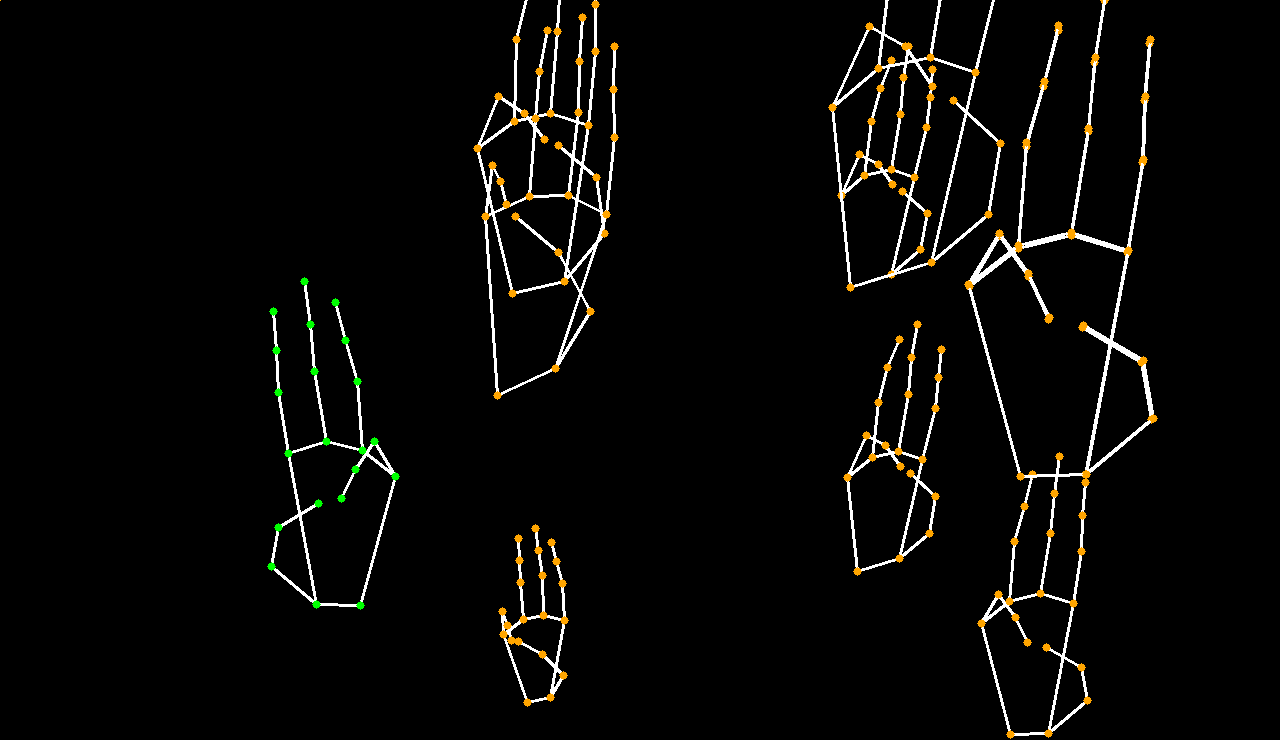
\includegraphics[width=0.5\linewidth]{material//figures/Augmentation.png}
    \caption{Augmentationpipeline Ergebnis (Original Grün | Augmented Orange)}
    \label{fig:augmentation}
\end{figure}

\subsection{Normalisierung und Interpolation}\label{sub:normalisierung}

Die extrahierten Landmarks werden für eine effiziente und positionsinvariante Darstellung normalisiert. Hierbei werden alle Landmark-Koordinaten relativ zum Handgelenk positioniert und in den INT16-Zahlenbereich ({-}32.768 bis 32.767) umgerechnet. Die Landmark-Daten werden als Dictionary mit den 21 benannten Schlüsseln und den zugehörigen \([x, y, z]\)-Koordinaten abgebildet. Zusätzlich wird die absolute Handgelenkposition (\texttt{wrist\_pos}) in Skalierung auf den INT16-Bereich sowie die Bounding-Box der Hand in Pixelkoordinaten (\texttt{hand\_area}) gespeichert. Die absoluten Landmark-Positionen in Pixelkoordinaten (\texttt{landmark\_pos}) werden ebenfalls erfasst.

Für eine einheitliche Darstellung aller Sequenzen erfolgt eine FPS-Normalisierung auf 60\,FPS mittels linearer Interpolation zwischen den Frames. Frames, in denen eine Hand nicht erkannt wird, werden durch leere Handstrukturen mit der Sentinel-Koordinate \([{-100}, {-100}]\) repräsentiert und bei der Interpolation als Sprungpunkte behandelt.

\subsection{Datenstrukturen und Speicherung}\label{sub:datenstrukturen}

Die verarbeiteten Geste- und Handdaten werden in den folgenden Datenstrukturen abgebildet:

Gesture: Repräsentation einer vollständigen Geste-Sequenz
\begin{itemize}
    \item label: Klasse der Geste (str)
    \item fps: Aktuelle Bildwiederholrate (float)
    \item frames: Liste von Frames, wobei jeder Frame eine Liste von zwei Hand-Objekten [left, right] enthält
\end{itemize}

Hand: Darstellung einer einzelnen Hand in einem Frame (frozen dataclass)
\begin{itemize}
    \item left\_hand: Seitenzugehörigkeit (bool)
    \item wrist\_pos: Absolute Handgelenkposition in int16-Skalierung \texttt{[x, y]}
    \item landmarks: Dictionary mit 21 benannten Landmarks relativ zum Handgelenk
    \item hand\_area: Bounding-Box in Pixelkoordinaten \texttt{(x, y, width, height)}
    \item landmark\_pos: Absolute Landmark-Positionen in Pixelkoordinaten (21 $\times$ \texttt{[x, y]})
\end{itemize}

Die verarbeiteten Geste-Daten werden im Pickle-Format (\texttt{.pkl}) abgelegt. Der Dateiname folgt dem Muster \texttt{\{Label\}\_\{Augmentierungstyp\}\_\{UUID\}.pkl}, wobei die UUID die ersten vier Hexadezimalzeichen eines UUID4 darstellt. Die Speicherung erfolgt im Verzeichnis \texttt{resources/gestures/}. Die Verarbeitung der Videodateien und die Speicherung der Ergebnisse werden mittels Multiprocessing unter Auslastung von 80\,\% der verfügbaren CPU-Kerne parallelisiert.

\section{Konfiguration und Training des Klassifikationsmodells}\label{sec:klassifikationsmodell}
\subsection{Problemdefinition}\label{sub:problemdefinition}

Das zu entwickelnde Modell soll die Fähigkeit besitzen, Gesten bestimmten Gruppen zuzuordnen. Eine Gruppe entspricht dabei immer einer Geste. Diese Einteilung von Datenpunkten (Gesten) in vordefinierte Klassen (Fingeralphabetzeichen) beschreibt Klassifikationsmodelle. Für jede Geste sollen die Wahrscheinlichkeiten für die zuzuordnenden Klassen ausgegeben werden.

Es liegt keine Binäreklassifikation vor, da mehr als zwei Klassen zu unterscheiden sind. Mit den 26 Klassen (NONE, A–Y ohne J und Z, SCH) handelt es sich um eine Multiklassen-Klassifikation.

\subsection{Datenanalyse}\label{sub:datenanalyse}

\paragraph{Input-Format:} Der Klassifikator empfängt einen 88-dimensionalen Feature-Vektor. Dieser setzt sich nach Ausgabe des Hand-Landmark Modells aus 44 Werten für die linke Hand (22 Gelenke $\times$ 2 Koordinaten) und 44 Werten für die rechte Hand (22 Gelenke $\times$ 2 Koordinaten) zusammen. Die 22 Gelenke pro Hand umfassen die 21 MediaPipe-Landmarks sowie die absolute Handgelenkposition. Koordinaten werden wrist-relativ normalisiert und auf den INT16-Bereich ({-}32.768 bis 32.767) skaliert.

\paragraph{Klassenverteilung:} Der Datensatz umfasst 26 Klassen: NONE (Index 0) für Keine Hand erkannt, A--Y (Indizes 1--24) für 24 statische Buchstaben (J und Z ausgeschlossen, da diese dynamische Handbewegungen erfordern) sowie SCH (Index 25) als Sonderzeichen. Die Klassenverteilung ist leicht ungleichmäßig (16 Klassen mit 185, 8 Klassen mit 148, NONE mit 111, F mit 110 Dateien).

\paragraph{Normalisierung:} Alle Koordinaten werden durch den Maximalwert des INT16-Bereichs \linebreak (POS\_MAX = 32.767) dividiert, sodass die Werte im Bereich \([{-}1, 1]\) liegen.

\subsection{Modellauswahl}\label{sub:modellauswahl}

Für die Modellauswahl wurden verschiedene Ansätze evaluiert, wobei die Anforderungen des eingebetteten Systems (schnelle Inferenz, kleine Modellgröße) und die Input-Struktur (88D-feature-Vektor aus MediaPipe-Landmarks) im Vordergrund standen.

Ein mehrschichtiges Perceptron (MLP) wurde als geeignetes Klassifikationsmodell ausgewählt. Ausschlaggebend hierfür war insbesondere die Struktur der Eingabedaten. Die vorgelagerte Landmark-Erkennung überführt die räumlichen Handinformationen in einen strukturierten Merkmalsvektor, sodass das Klassifikationsmodell nicht das vollständige Kamerabild verarbeitet. Fritz zeigt, dass unterschiedliche Klassifikatoren auf Grundlage solcher MediaPipe-Landmarks hohe Erkennungsleistungen erreichen können. Das untersuchte CNN erzielte zwar eine etwas höhere Genauigkeit als das MLP, erforderte jedoch erheblich mehr Speicherressourcen. Für die ressourcenbeschränkte Zielplattform wurde daher ein MLP als Kompromiss zwischen Klassifikationsleistung und Modellkomplexität gewählt \cite[S. 57 ff.]{fritzHandGestureRecognition}.

Random Forest und SVM wurden ebenfalls in Betracht gezogen, erreichen jedoch in der Literatur geringere Genauigkeiten (70–75\% bzw. 61–76\%) bei vergleichbaren Tasks. Zudem fehlen beiden Modellen nativ kalibrierte Wahrscheinlichkeiten: Random Forest gibt nur harte Klassifikationen aus, während SVM ein zusätzliches Platt-Scaling für Wahrscheinlichkeiten erfordert. \cite{rahmanComparisonSVMRandom2025}. Es ist anzumerken das SVM und Random Forest auf einer anderen Datenbasis (Photoplethysmography (PPG)) trainiert worden sind.

Das MLP erfüllt die Anforderungen an Ressourcenbeschränkungen und Echtzeitfähigkeit.
Die Softmax-Ausgabeschicht liefert direkt die für die nachfolgende Verarbeitung benötigten
Klassenwahrscheinlichkeiten. Während eine direkte Quantisierung zu Genauigkeitsverlusten
führen kann, zeigen Untersuchungen, dass geeignete Quantisierungsverfahren eine
INT8-Inferenz bei weitgehend erhaltener Modellgenauigkeit ermöglichen
\cite{jacobQuantizationTrainingNeural2018}. Dies stellt einen akzeptablen Kompromiss
für den Embedded-Einsatz dar.

\subsection{Modellarchitektur}\label{sub:modellarchitektur}

\begin{figure}[!htbp]
    \centering
    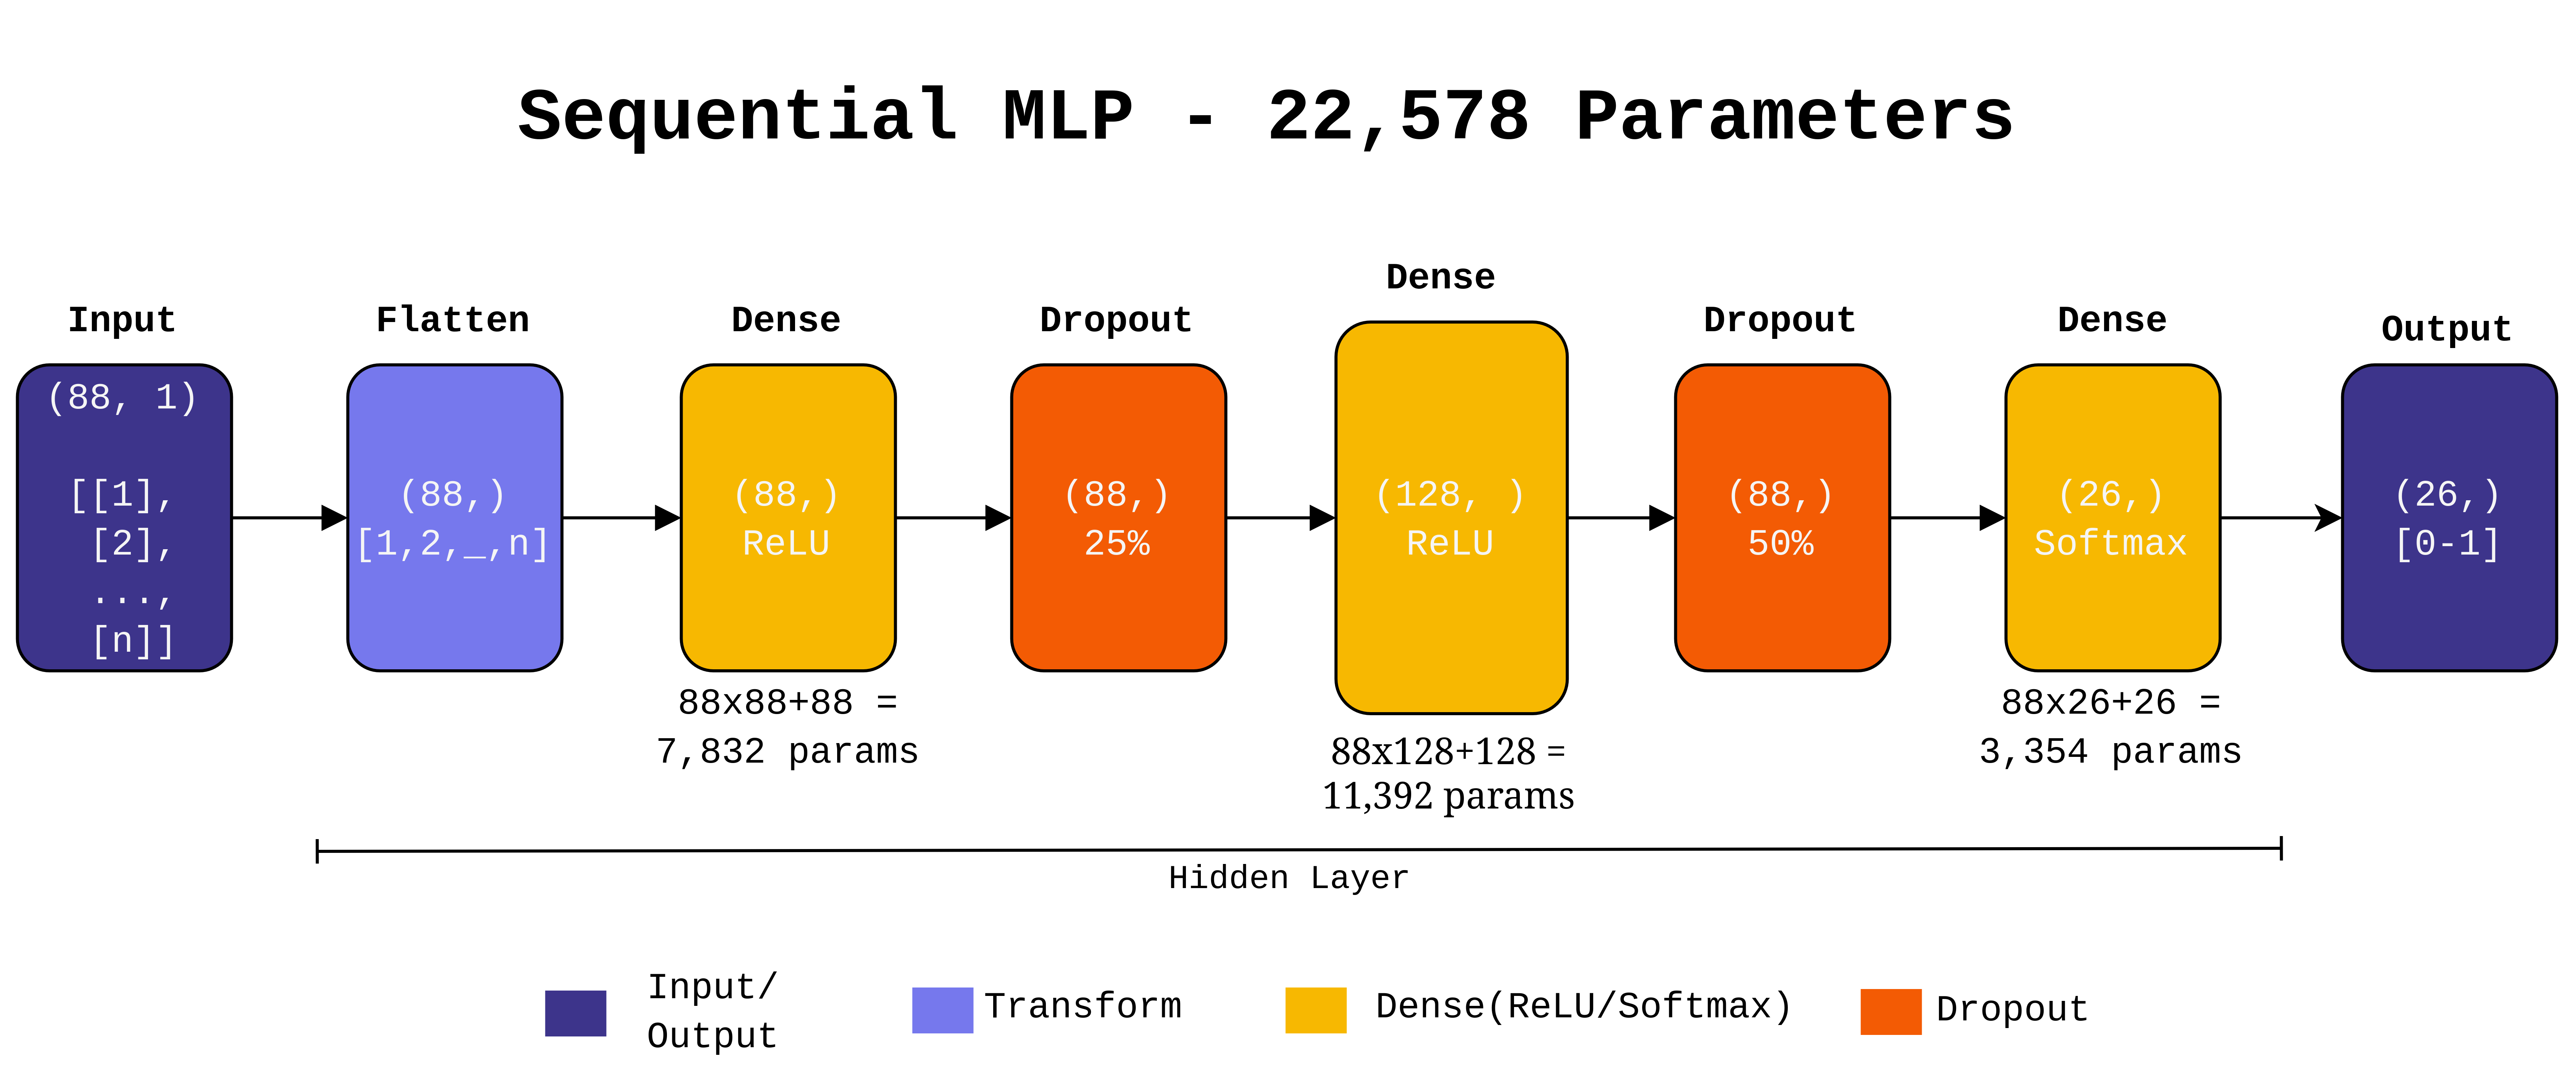
\includegraphics[width=0.8\textwidth]{material/figures/Sequential MLP.drawio.png}
    \caption{Architektur des Multi-Layer Perceptrons | Eigene Darstellung}
    \label{fig:mlp-architektur}
\end{figure}

Das Klassifikationsmodell setzt sich aus sieben Schichten zusammen, die sequenziell eine direkte Informationsflussrichtung von der Eingabe zur Ausgabe aufweisen. Die Architektur folgt dem Prinzip der schrittweisen Transformation und Abstraktion der Eingabemerkmale. Nachdem der Input-Tensor in eine eindimensionale Darstellung überführt wurde, transformiert die erste Dense-Schicht die Rohmerkmale in einen repräsentativen Feature-Raum. Die nachfolgende Dense-Schicht erweitert diesen Raum, um komplexere Inter-Feature-Beziehungen modellieren zu können. Zwischen den Dense-Schichten werden Dropout-Schichten eingebunden um Zufall in das Modell zu bringen, um Overfitting zu verhindern. Die finale Dense-Schicht projeziert die gelernten Repräsentationen auf die 26 Ausgabeklassen.

Der Input-Layer empfängt einen tensor der Form \texttt{(88,1)}. Dieser Tensor repräsentiert die normalisierten Merkmale zweier Hände mit je 44 Werten. Pro enthalten sind 21 MediaPipe-Hand-Landmarks jeweils als \texttt{(x,y)}-Koordinate sowie die absolute Handgelenkposition ebenfalls als \texttt{(x,y)}. Alle Koordianten sind Handgelenksrelativ normalisiert und auf den int15-Bereich skaliert, sodass der Input-Wertebereich [-1, 1] beträgt.

Der Flatten-Layer überführt den mehrdimensionalen Input-Tensor in einen eindimensionalen Vektor der Länge 88. Dense-Schichten erwarten als Eingabe einen flachen Vektor, sodass die räumliche Struktur des Tensors (2 Hände x 44 Werte) für die nachfolgende Gewichtsmatrix aufgelöst werden kann.

Der erste Dense-Layer mit 88 Neuronen und ReLU-Aktivierung (vgl.\ Abschnitt~\ref{sub:aktivierungsfunktionen}) führt per-Feature-Transformationen durch. Das bedeutet durch die  Gewichtsmatrix (88×88) und den Bias-Vektor wird jedes Eingabemerkmal einzeln transformiert. Die ReLU-Aktivierung fügt Nicht-Linearität hinzu und ermöglicht es dem Modell, nicht-triviale Muster in den Landmark-Daten zu erkennen. Die Wahl von 88 Neuronen hält die Kapazität zunächst auf gleicher Dimension wie der Input und zwingt das Modell, die Merkmale in einem äquivalenten Raum abzubilden, bevor eine Dimensionserweiterung erfolgt.

Der Dropout-Layer (0.25) deaktiviert während des Trainings zufällig 25\% der Ausgaben des vorherigen Dense-Layers. Die zufällige Deaktivierung von Neuronen dient der Regularisierung und verhindert das Overfitting des Modells (vgl.\ Abschnitt~\ref{sub:overfitting}). Jedes Neuron wird mit einer Wahrscheinlichkeit von 0.25 auf den Wert 0 gesetzt. \cite{yingOverviewOverfittingIts2019}

Der zweite Dense-layer mit 128 Neuronen und ReLU-Aktivierung erweitert den Feature-Raum von 88 auf 128 Dimensionen. Durch die Erhöhung der Kapazität kann des Modell Inter-Feature-Beziehungen modellieren, die über die per-Feature-Transformationen des vorherigen Layers hinausgehen. Typische Beziehungen umfassen:

\begin{itemize}

    \item Intra-Hand-Abhängigkeiten: Korrelation zwischen benachbarten Landmarks des selben Fingers (z.B. die Auslenkung von PIP und DIP des Indexfingers), zwischen verschiedenen Fingern einer Hand sowie  die Orientierung der Hand und deren Rotation basierend auf der Handflächen features.
    \item Inter-Hand-Beziehungen: Zusammenhänge zwischen den Landmarks beider Hände, die bei einhändigen Gesten durch symmetrische oder asymmetrische Konfigurationen entstehen können.
    \item Komplexe Muster: Nicht-lineare Kombinationen mehrerer Landmarks, die erst in der erweiterten Repräsentation als discriminative Merkmale erkennbar werden.
\end{itemize}

Der zweite Dropout-Layer (0.5) wendet eine stärkere Regularisierung an als der erste \linebreak Dropout-Layer. Die Rate von 50\% ist bewusst höher gewählt, da der vorherige Dense-Layer mit 128 Neuronen eine größere Modellkapazität aufweist und die Gefahr des Overfitting steigt. Die stärkere Regularisierung vor der Ausgabeschicht stellt sicher, dass das Modell nur die robustesten Feature-Repräsentationen für die finale Klassifikation verwendet.

Der dritte Dense-Layer mit 26 Neuronen und Softmax-Aktivierung bildet die finale Klassifikationsschicht. Die 26 Ausgabeneuronen entsprechen den 26 Klassen (NONE, A–Y ohne J und Z, SCH). Die Softmax-Funktion (vgl.\ Abschnitt~\ref{sub:aktivierungsfunktionen}) normalisiert die Rohausgaben (Logits) in Wahrscheinlichkeiten, deren Summe exakt eins ergibt. Jedes Ausgabeneuron liefert damit die Wahrscheinlichkeit dafür, dass der Input der entsprechenden Gebärdensprache-Klasse angehört.

\subsection{Verlustfunktion und Optimierung}\label{sub:verlustfunktion}

Für das Training des Modells wird die Verlustfunktion Sparse Categorical Crossentropy verwendet, die bereits in Abschnitt~\ref{ssub:sparse-cce} eingeführt wurde. Sie eignet sich insbesondere, da die Zielklassen als Integer und nicht als One-Hot-Vektoren kodiert vorliegen. Die Verlustfunktion berechnet die Abweichung zwischen den tatsächlichen Klassen und den durch die Softmax-Ausgabe vorhergesagten Klassenwahrscheinlichkeiten und lässt sich durch folgende Formel beschreiben:
$$L = -\log(p_{y_{true}})$$
wobei $p_{y_{true}}$ die vom Modell vorhergesagte Wahrscheinlichkeit der tatsächlichen Klasse bezeichnet. \cite{WhatSparseCategorical10:49:00+00:00}

\subsection{Trainingsprozess}\label{sub:trainingsprozess}

Um einen Trainingsprozess durchlaufen zu können müssen Hyperparameter bestimmt werden (vgl.\ Abschnitt~\ref{sub:parameter-hyperparameter}). Zentral sind Optimizer, Lernrate, Verlustfunktion, Epochen, Trainingssplit, Batch Size und Frühzeitiges Stoppen.

Als Optimizer wird Adam (Adaptive Moment Estimation) verwendet, dessen Funktionsweise in Abschnitt~\ref{sub:optimierung-training} erläutert wurde. Adam kombiniert die Vorteile von Momentum und adaptiven Lernraten und konvergiert dadurch in der Regel schneller und stabiler als klassische Optimierungsverfahren wie Stochastic Gradient Descent (SGD). Insbesondere bei kleinen oder mittelgroßen Datensätzen sowie komplexen neuronalen Netzen liefert Adam häufig robuste Ergebnisse, da weniger aufwendige Hyperparameteranpassungen erforderlich sind. \cite{a.g.TuningHyperparameterADAM2026}

Die Lernrate (siehe Abschnitt~\ref{sub:optimierung-training}) bestimmt die Größe der Aktualisierungsschritte während der Optimierung. Eine sehr kleine Lernrate von $10^{-5}$ reduziert das Risiko, das Minimum der Verlustfunktion zu überschreiten oder instabile Trainingsverläufe zu erzeugen. Der Nachteil einer geringeren Lernrate besteht in einer längeren Trainingsdauer, die jedoch durch eine stabilere Konvergenz ausgeglichen wird.

Als Verlustfunktion dient die in Abschnitt~\ref{sub:verlustfunktion} eingeführte Sparse Categorical Crossentropy. Im Gegensatz zur Categorical Crossentropy ist keine One-Hot-Kodierung der Labels erforderlich, wodurch Speicherbedarf und Vorverarbeitungsaufwand reduziert werden.

Die Sparse categorical Accuracy Metrik gibt den Anteil der korrekt klassifizierten Beispiele an und stellt damit eine leicht interpretierbare Leistungskennzahl dar (vgl.\ Abschnitt~\ref{sub:metriken}). Da die Zielklassen als Integer vorliegen, passt sie direkt zur verwendeten Verlustfunktion SparseCategoricalCrossentropy. Während die Verlustfunktion zur Optimierung dient, ermöglicht die Accuracy eine intuitive Bewertung der Modellleistung während des Trainings und auf den Validierungsdaten.

Eine Epoche entspricht einem vollständigen Durchlauf des Trainingsdatensatzes (siehe Abschnitt~\ref{sub:optimierung-training}). Die Wahl von 20 Epochen bietet dem Modell ausreichend Möglichkeiten, die zugrunde liegenden Muster zu erlernen, ohne die Trainingszeit unnötig zu verlängern. Da zusätzlich Early Stopping eingesetzt wird, dient dieser Wert als maximale Obergrenze. Das Training endet automatisch früher, sobald keine Verbesserung der Validierungsleistung mehr festgestellt wird.

Ein weiterer Hyperparameter ist die Aufteilung der Trainingsdaten in Training, Validation und Testdaten. Durch die Aufteilung des Datensatzes in 64\% Trainingsdaten, 16\% Validierungsdaten und 20\% Testdaten kann die Generalisierungsfähigkeit des Modells während des Trainings überprüft werden. Die Validierungsdaten werden nicht für das Lernen verwendet und ermöglichen daher eine unabhängige Beurteilung der Modellleistung.

Die Batch Size legt fest, wie viele Trainingsbeispiele gleichzeitig verarbeitet werden, bevor eine Aktualisierung der Modellgewichte erfolgt (siehe Abschnitt~\ref{sub:optimierung-training}). Eine Batchgröße von 128 stellt einen guten Kompromiss zwischen Rechenleistung, Speicherbedarf und Trainingsstabilität dar. Größere Batches ermöglichen eine effizientere Nutzung von GPU Hardware dar und liefern stabile Gradienten, während kleinere Batches zwar stärkeres Rauschen erzeugen, jedoch teilweise eine bessere Generalisierung fördern. Die gewählte Batchgröße bietet daher eine ausgewogene Balance zwischen Trainingsgeschwindigkeit und Modellqualität.

Early Stopping dient der Vermeidung von Overfitting und beendet das Training vorzeitig, sobald sich die Validierungsleistung über mehrere Epochen nicht mehr verbessert (vgl.\ Abschnitt~\ref{sub:optimierung-training}). Mit einer Patience von drei werden kleinere Schwankungen der Validierungsverluste toleriert, bevor das Training gestoppt wird. Dadurch wird verhindert, dass unnötig lange trainiert wird oder das Modell beginnt, sich zu stark an die Trainingsdaten anzupassen. Gleichzeitig wird das Modell mit der besten Validierungsleistung gespeichert bzw. verwendet.


\begin{longtable}{|p{0.35\textwidth}|p{0.55\textwidth}|}
    \hline
    \textbf{Parameter} & \textbf{Wert} \\
    \hline
    \endfirsthead
    \hline
    \textbf{Parameter} & \textbf{Wert} \\
    \hline
    \endhead
    \hline
    \multicolumn{2}{r}{\texttt{Fortsetzung auf nächster Seite}} \\
    \endfoot
    \caption{Hyperparameter des Modelltrainings}
    \label{tab:hyperparameter} \\
    \endlastfoot
    Optimizer & Adam \\
    \hline
    Learning Rate & 0,00001 \\
    \hline
    Verlustfunktion & Sparse Categorical Crossentropy \\
    \hline
    Metrik & Sparse Categorical Accuracy \\
    \hline
    Epochen & 20 \\
    \hline
    Validation Split & 0,2 (80/20) \\
    \hline
    Batch Size & 128 \\
    \hline
    Early Stopping & 3 \\
    \hline
\end{longtable}

\section{Quantisierung, Konvertierung und Deployment der Modelle}\label{sec:quantisierung-deployment}

Das folgende Kapitel beschreibt die Quantisierung des Tensorflow Fingeralphabet Modells, die Convertierung der Quantisierten Handdedektion-, Landmarkerkennung- und Fingeralphabet- Modelle in NPU ausführbare Binaries. Im letzten Schritt wird das Flashen der Modelle auf den STM32N650DK beschrieben.

\newpage
\subsection{Quantisierung von Tensorflow Modellen}\label{sub:quantisierung-tf}

Der folgende Codeausschnitt zeigt den vollständigen Ablauf der Konvertierung vom trainierten Keras-Modell bis zur gespeicherten INT8-TFLite-Datei:
\begin{lstlisting}[language=python, caption={Vollständige INT8-Quantisierung des Fingeralphabet-Modells}, label={lst:tflite-quantisierung}]
model = keras.models.load_model(MODEL_DIR)
converter = tf.lite.TFLiteConverter.from_keras_model(model)

converter.optimizations = [tf.lite.Optimize.DEFAULT]

def representative_dataset():
    """Liefert Kalibrierungsdaten im Eingabeformat des Modells (88, 1)."""
    try:
        data = pickle.load(open(TRAINING_DATA_PATH, "rb"))
        inputs = data.training_inputs.reshape(-1, 88, 1)
        for i in range(min(len(inputs), 500)):
            yield [inputs[i:i + 1]]
    except (FileNotFoundError, AttributeError, pickle.UnpicklingError):
        for _ in range(100):
            yield [np.random.uniform(-1.0, 1.0, (1, 88, 1)).astype(np.float32)]

converter.representative_dataset = representative_dataset

converter.target_spec.supported_ops = [tf.lite.OpsSet.TFLITE_BUILTINS_INT8]
converter.inference_input_type = tf.uint8
converter.inference_output_type = tf.uint8

tflite_model = converter.convert()
with open("model_int8.tflite", "wb") as f:
    f.write(tflite_model)
\end{lstlisting}

Zuerst wird das trainierte Keras-Modell geladen und ein TensorFlow-Lite-Konverter erzeugt. Anschließend aktiviert \texttt{converter.optimizations = [tf.lite.Optimize.DEFAULT]} \linebreak die  Standardoptimierungen, die eine verlustbehaftete Post-Training-Quantisierung ermöglichen (siehe Abschnitt~\ref{sub:modellquantisierung}).

Für die Kalibrierung wird mit \texttt{converter.representative\_dataset} ein repräsentativer Datensatz bereitgestellt, wie er in Abschnitt~\ref{sub:modellquantisierung} beschrieben wurde. Während der Kalibrierung bestimmt TensorFlow Lite anhand dieser Daten die Wertebereiche der Aktivierungen, um geeignete Skalierungsfaktoren und Nullpunkte für die Quantisierung zu berechnen. Sind die Trainingsdaten nicht verfügbar, wird ersatzweise ein Datensatz aus gleichverteilten Zufallswerten im Bereich $[-1, 1]$ verwendet.

Da die Zielhardware ausschließlich INT8-Operationen unterstützt, wird die Konvertierung \linebreak durch \texttt{TFLITE\_BUILTINS\_INT8} entsprechend eingeschränkt und der Ein- und Ausgabedatentyp des Modells auf 8-Bit-Ganzzahlen festgelegt. Abschließend wird das Modell mit \linebreak \texttt{converter.convert()} in das TensorFlow-Lite-Format konvertiert und als \texttt{.tflite}-Datei gespeichert. Ergebnis ist ein vollständig quantisiertes TensorFlow-Lite-Modell, das den Anforderungen der eingesetzten NPU entspricht und anschließend mit STEdgeAI in eine für das Embedded-System ausführbare Binärdatei überführt werden kann. Durch die Quantisierung werden der Speicherbedarf und der Rechenaufwand reduziert, während die Modellgenauigkeit durch die Verwendung repräsentativer Kalibrierungsdaten weitgehend erhalten bleibt.

\subsection{Konvertierung INT8-Quantisierte-Modelle zu Embedded binaries}\label{sub:konvertierung}

Nach der Quantisierung liegen alle drei Modelle (Handdetektion, Handlandmark-Erkennung und Fingeralphabet-Klassifikation) im TensorFlow-Lite-Format mit einer INT8-Quantisierung vor. Der nächste Verarbeitungsschritt ist diese Modelle mithilfe der ST Edge AI Core CLI (Kapitel ~\ref{sub:stedge-ai}) in für die Zielhardware ausführbare Binärdateien zu überführen. Die Verwendung der Kommandozeilenschnittstelle (CLI) wurde bewusst der grafischen Benutzeroberfläche (GUI) vorgezogen, da sich hierdurch der gesamte Konvertierungsprozess automatisieren lässt. Auf diese Weise können Skripte erstellt werden, welche die Generierung aller Modellartefakte reproduzierbar und mit einem einzelnen Aufruf durchführen.

Die Verzeichnisstruktur der Modellgenerierung:

\begin{lstlisting}[language=bash, numbers=none, caption={Verzeichnisstruktur der Modellgenerierung}, label={lst:model-dir-structure}]
models/
+-- source/                           <- Raw TFLite models (input)
|   +-- 033_palm_detection_full_quant_pc_ff_od.tflite
|   +-- 033_hand_landmark_full_quant_pc_uf_handl.tflite
|   \-- fingeralphabet_model_int8.tflite
|
+-- my_mpools/                        <- Memory pool definitions per model
|   +-- palm_detection.mpool
|   +-- hand_landmark.mpool
|   \-- fingeralphabet.mpool
|
+-- user_neuralart.json   <- Per-model config (links model -> mpool+compiler flags)
+-- generate_n6_models.sh <- Orchestrator script (calls stedgeai, copies outputs)
+-- copy_n6_models.sh     <- Copies generated files into the firmware project tree
|
+-- generated/            <- Output: C source + headers ready for compilation
|   +-- palm/
|   +-- landmark/
|   \-- finger/
|
\-- st_ai_output/         <- Intermediate build artifacts (gitignored)
\end{lstlisting}

\paragraph{Modell Profile}

In der Struktur definiert \texttt{user\_neuralart.json} wie die einzelnen Modelle bei der Compilierung für die STM32N6 NPU zu behandeln sind. Sie enthält einen Abschnitt \texttt{Profiles} mit jeweils einem Eintrag pro Modell:

\begin{lstlisting}[language=json, caption={Modellprofil in user\_neuralart.json}, label={lst:user-neuralart}]
{
  "Profiles": {
    "palm_detection_model_v3": {
      "memory_pool": "./my_mpools/palm_detection.mpool",
      "options": "--enable-epoch-controller"
                 "-O3"
                 "--all-buffers-info"
                 "--cache-maintenance"
    }
  }
}
\end{lstlisting}

\texttt{memory\_pool} \newline
Verweist auf die \texttt{.mpool}-Datei, die das Speicherlayout der NPU für dieses Modell definiert (welche SRAM-Bänke, Flash-Bereiche, Adressen und Größen).

\texttt{options} \newline
Definiert pro Modell welche Compilerflags verwendet werden sollen. Folgend werden verwendete Compiler flags in \ref{tab:stedgeai-flags} kurz erläutert.

\begin{longtable}{|p{0.3\textwidth}|p{0.65\textwidth}|}
    \hline
    \textbf{Flag} & \textbf{Effekt} \\
    \hline
    \endfirsthead
    \hline
    \textbf{Flag} & \textbf{Effekt} \\
    \hline
    \endhead
    \hline
    \multicolumn{2}{r}{\texttt{Fortsetzung auf nächster Seite}} \\
    \endfoot
    \caption{ST Edge AI Core Compiler Flags}
    \label{tab:stedgeai-flags} \\
    \endlastfoot
    --enable-epoch-controller & Ermöglicht die epochenbasierte Ausführung der NPU (schichtweise Ablaufplanung) \\
    \hline
    -O3/-O2 & Optimierungsstufe für den NPU-Codegenerator \\
    \hline
    --all-buffers-info & Vollständige Puffer-Metadaten für die Laufzeit ausgeben \\
    \hline
    --cache-maintenance / --Ocache-opt & Befehle zum Leeren / Ungültig machen des Caches einfügen \\
    \hline
    --Oauto-sched & Automatisches planen der Epochen (default/Ohne Verweis) \\
    \hline
    --native-float & Verwendet Hardware-Float-Operationen wenn möglich \\
    \hline
    --enable-virtual-mem-pools & Erlaubt dem Linker Tensoren über mehrere physische Speicherregionen zu verteilen \\
    \hline
    --Omax-ca-pipe \texttt{<num>} & Legt die maximale Anzahl an Compute- \& Accumulate-(CA-) Pipelines bzw.\ parallelen Hardware-Ausführungspfaden fest, die der Compiler gleichzeitig zuweisen darf. \\
    \hline
    --Oconv-split-kw & Aufteilen von Faltungskernen auf die verfügbaren NPU-MAC-Arrays \\
    \hline
\end{longtable}

\paragraph{Memory-Pool-Definition}
Die \texttt{.mpool}-Dateien beschreiben die STM32N6 Hardware Speicherabbild der NPU. Alle \texttt{.mpool}-Dateien haben den identischen Aufbau. Der einzige wesentliche Unterschied zwischen den Modellen besteht in der xSPI2 (flash) Region (Basisadresse und Größe) an welcher die Modelle gespeichert sind.

Ein Hauptbereich ist die \texttt{params}-Sektion, welche die maximale verfügbare On-Chip-SRAM-Größe auf 1024\,KB für die NPU beschränkt.

\begin{lstlisting}[language=json, caption={Globale Speicher einschränkung in .mpool}, label={lst:mpool-params}]
{ "paramname": "max_onchip_sram_size", "value": "1024", "magnitude": "KBYTES"}
\end{lstlisting}

Weitere Sektionen sind \texttt{cacheinfo} und \texttt{mempools}.  Diese beschreiben den zu nutzenden Cache, bzw. die Speicherbereich-Konfiguration pro Modell auf der NPU. Diese ist wie folgt zugeteilt:

\begin{longtable}{|l|l|l|l|p{0.3\textwidth}|}
    \hline
    \textbf{Name} & \textbf{Region} & \textbf{Adresse} & \textbf{Größe} & \textbf{Rolle} \\
    \hline
    \endfirsthead
    \hline
    \textbf{Name} & \textbf{Region} & \textbf{Adresse} & \textbf{Größe} & \textbf{Rolle} \\
    \hline
    \endhead
    \hline
    \multicolumn{5}{r}{\texttt{Fortsetzung auf nächster Seite}} \\
    \endfoot
    \caption{NPU-Speicherbereich-Konfiguration}
    \label{tab:npu-mempools} \\
    \endlastfoot
    npuRAM3 & AXISRAM3 & 0x34200000 & 448\,KB & NPU activation scratch \\
    \hline
    npuRAM4 & AXISRAM4 & 0x34270000 & 448\,KB & NPU activation scratch \\
    \hline
    npuRAM5 & AXISRAM5 & 0x342e0000 & 448\,KB & NPU activation scratch \\
    \hline
    npuRAM6 & AXISRAM6 & 0x34350000 & 448\,KB & NPU activation scratch \\
    \hline
    hyperRAM & xSPI1 & 0x90000000 & 0\,MB & External HyperRAM (Deaktiviert) \\
    \hline
    octoFlash & xSPI2 & 0x71000000 & 2\,MB & Weight storage in OctoSPI flash \\
    \hline
\end{longtable}

Die vier AXISRAM-Bänke sind On-Chip-SRAM-Speicher mit hohem Durchsatz und geringer Latenz, die für Laufzeit-Aktivierungen (Zwischentensoren) genutzt werden. \texttt{octoFlash} ist zur Laufzeit schreibgeschützt (ACC\_READ) und speichert die Modellgewichte bzw.\ -konstanten. Die Einstellung \texttt{constants\_preferred: "true"} weist das Tool an, konstante Daten in diesem Bereich abzulegen.

Die Flash-Basisadressen unterscheiden sich je nach Modell, um den 16-MB-xSPI2-Flash zu partitionieren:

\begin{table}[htbp]
    \centering
    \begin{tabular}{|l|l|l|}
        \hline
        \textbf{Modell} & \textbf{Flash Start} & \textbf{Flash Size} \\
        \hline
        Finger & \texttt{0x71000000} & 2\,MB \\
        \hline
        Handdetektion & \texttt{0x71200000} & 4\,MB \\
        \hline
        Handlandmark & \texttt{0x71600000} & 10\,MB \\
        \hline
    \end{tabular}
    \caption{Flash-Partitionierung je Modell}
    \label{tab:flash-partitionierung}
\end{table}

\paragraph{Script - Generierung}
Das \texttt{generate\_n6\_models.sh}-Script führt für jedes Modell 3 Schritte durch (Konvertierung, Kopieren und Project-Build). Im ersten Schritt wird die ST Edge AI Core CLI zur Konvertierung \texttt{TF-Lite $\rightarrow$ NPU-Artefakte} verwendet.

\begin{lstlisting}[language=bash, caption={STedgeAI Modellgenerierung}, label={lst:stedgeai-generate}]
stedgeai generate \
    --name palm_detection_model_v3 \
    --model source/033_palm_detection_full_quant_pc_ff_od.tflite \
    --target stm32n6 \
    --st-neural-art "palm_detection_model_v3@user_neuralart.json" \
    --input-data-type uint8 \
    --output st_ai_output/
\end{lstlisting}

Dies liest das TensorFlow-Lite-Modell ein, lädt die \texttt{palm\_detection\_model\_v3} Konfiguration in \texttt{user\_neuralart.json} um den Memory-Pool und Compiler-Optionen zu erhalten und generiert Gewichtsdaten als C-Arrays, entsprechende Header mit Attributen für Linker-Sek-tionen, ST-AI-Runtime-API-Wrapper und einen Binär-Blob mit Gewichten zur Flash-Programm-ierung. Die genaue Aufspaltung ist in Kapitel \ref{sub:modell-aufsplittung}.

Der zweite Schritt Konvertiert \texttt{.raw} Gewichts-Blob in eine Intel \texttt{.hex}-Datei mit der korrekten Basisadresse (z.\,B.\ 0x71000000). Diese Hex-Datei kann via STM32CubeProgrammer auf den Mikrocontroller geflashed werden.

Der lertzte Schritt führt das \texttt{copy\_n6\_models.sh}-Script aus. Es kopiert die generierten Dateien in das STM32N6570DK-Embedded-Projekt:
\begin{itemize}
    \item \texttt{*.c} und \texttt{*\_ecblobs.h} $\rightarrow$ \texttt{embedded/STM32N6570DK/FSBL/Src/AI/\textless Model\textgreater/Src/Inc/}
    \item \texttt{stai\_\*.c/h} (with \texttt{--stai} flag)
    \item \texttt{*.bin} weight blobs (with \texttt{--weights} flag) $\rightarrow$ \texttt{FSBL/Assets/AI/}
\end{itemize}

Zudem wird \texttt{\*\_ecblobs.h} gepatcht, um \verb|#include "ecblob_sections.h"| einzufügen. Dadurch wird sichergestellt, dass die Gewichts-Arrays im ECBLOBS-Linker-Abschnitt landen, anstatt des internen ROM (2047\,KB) zu sprengen.

% ============================================================================
% Speicherarchitektur, Modell-Aufsplittung und Flash-Layout des STM32N6570-DK
% Quellen:
%   - embedded/Memory Map.md
%   - embedded/Sign_Language_Translator/STM32N657X0HXQ_AXISRAM2_fsbl.ld
%   - embedded/Sign_Language_Translator/flash_models.sh
%   - generierte Modelldateien (*_model_v3.c, *_model_v3_ecblobs.h, *.mpool)
% ============================================================================
\subsection{Aufsplittung der Modelle}\label{sub:modell-aufsplittung}

Die drei verwendeten Modelle (Fingeralphabet-Klassifikation, Handdetektion und
Hand- \linebreak landmark-Erkennung) werden mit dem ST Edge AI Core Compiler nicht als ein zusammenhängendes Artefakt erzeugt. Das Resultat ist in mehrere getrennte Speicherobjekte aufgesplittet. Ursache hierfür ist die Speicherhierarchie des STM32N6570: Der Chip besitzt keinen internen Flash, lediglich ca.\ 4{,}2\,MB On-Chip-SRAM, zwei externe Speicherschnittstellen
(XSPI1/PSRAM, XSPI2/NOR-Flash) sowie einen dedizierten NPU-Beschleuniger.
Ein kompiliertes Modell zerfällt daher in die folgenden vier Bestandteile:

\begin{enumerate}
  \item Gewichte und Konstanten: Die Quantisierungs- und Gewichtsdaten werden vom Compiler als roher Binär-Blob (\texttt{*\_atonbuf.xSPI2.bin}) ausgegeben. Der Namenszusatz \texttt{xSPI2} verweist auf den Speicherpool \texttt{octoFlash}, dem die Konstanten durch die \texttt{.mpool}-Konfiguration zugewiesen werden. Der Pool ist zur Laufzeit schreibgeschützt (\texttt{ACC\_READ}) und mit \texttt{constants\_preferred: true} markiert, sodass der Compiler alle konstanten Daten dort ablegt. Die Gewichte werden im externen NOR-Flash abgelegt und von der NPU über ihren AXI-Cache als Datenströme gelesen.

  \item EC-Blobs (Epoch-Controller-Blobs): Zusätzlich zu den Gewichten erzeugt der Compiler pro ausgeführter Epoche einen Microinstruktions-Blob, der den Epoch Controller der NPU schichtweise ablaufen lässt. Diese Blobs werden als C-Arrays in den Dateien \texttt{*\_model\_v3\_ecblobs.h} generiert. Über die Attribute \texttt{ECBLOB\_CONST\_SECTION} und \texttt{ECBLOB\_RUNTIME\_SECTION} (siehe \texttt{ecblob\_sections.h}) werden sie den Linker- \linebreak Abschnitten \texttt{.ecblobs\_const} bzw. \texttt{.ecblobs\_runtime} zugeordnet und damit in die On-Chip-SRAM Regionen \texttt{EC\_CONST} und \texttt{EC\_RUNTIME} eingebettet. Tabelle~\ref{tab:ecblob-umfang} fasst die Anzahl und Größe der Konstanten-Blobs je Modell zusammen.

  \item Aktivierungsdaten (Zwischentensoren): Die während der Inferenz anfallenden Aktivierungen werden vom Compiler auf die vier NPU-tauglichen SRAM-Bänke \texttt{AXISRAM3} bis \texttt{AXISRAM6} (in der NPU-Konfiguration \texttt{npuRAM3} bis \texttt{npuRAM6}, je 448\,KB) verteilt. Das Compiler-Flag \texttt{--enable-virtual-mem-pools} erlaubt dabei das Verteilen einzelner Tensoren über mehrere physische Speicherregionen (virtuelle Pools).

  \item Ein- und Ausgabepuffer: Die Eingabebilder der Modelle (\texttt{nn\_in}, z.\,B.\ 192$\times$192\,px für die Handdetektion) und die Ausgabetensoren (\texttt{nn\_out}, z.\,B.\ Heatmaps der Handlandmark-Erkennung) werden als benutzerspezifische Puffer in RAM beziehungsweise in die dafür vorgesehenen AXISRAM-Bänke gelegt.
\end{enumerate}

\begin{table}[htbp]
  \centering
  \label{tab:ecblob-umfang}
  \begin{tabular}{lrrr}
    \toprule
    Modell & Blobs & Blob-Größe & Anteil an EC\_CONST (512\,KB) \\
    \midrule
    Fingeralphabet   &  2 & 8\,320\,B   ($\approx$ 8{,}1\,KiB)  & 1{,}6\,\% \\
    Handdetektion    &  8 & 321\,216\,B ($\approx$ 313{,}7\,KiB) & 61{,}3\,\% \\
    Handlandmark     &  2 & 140\,288\,B ($\approx$ 137{,}0\,KiB) & 26{,}8\,\% \\
    \midrule
    Gesamt           & 12 & 469\,824\,B ($\approx$ 458{,}8\,KiB) & \textbf{89{,}6\,\%} \\
    \bottomrule
  \end{tabular}
  \caption{Umfang der Epoch-Controller-Blobs (\texttt{.ecblobs\_const}) je Modell}
\end{table}

% ============================================================================
\section{Speicherbelegung}

\subsection{Linker-Region-Definitionen}\label{sec:linker-belegung}

Die Speicheraufteilung wird im Linker-Skript
\texttt{STM32N657X0HXQ\_AXISRAM2\_fsbl.ld} über die \texttt{MEMORY}-Regionen
festgelegt. Tabelle~\ref{tab:linker-regionen} listet die Regionen mit ihrer
reservierten Größe und der tatsächlich belegten Größe auf:

\begin{longtable}{l l l r r}
    \hline
    \textbf{Region} & \textbf{Basisadresse} & \textbf{reserviert} & \textbf{tatsächlich belegt} & \textbf{Auslastung} \\
    \hline
    \endfirsthead
    \hline
    \textbf{Region} & \textbf{Basisadresse} & \textbf{reserviert} & \textbf{tatsächlich belegt} & \textbf{Auslastung} \\
    \hline
    \endhead
    \hline
    \multicolumn{5}{r}{\texttt{Fortsetzung auf nächster Seite}} \\
    \endfoot
    \caption{Tatsächliche Speicherbelegung der Linker-Regionen}
    \label{tab:linker-regionen} \\
    \endlastfoot
    ROM         & \texttt{0x34000400} & 2047\,KB & aus \texttt{.map} & -- \\
    \hline
    RAM         & \texttt{0x34180000} & 512\,KB  & aus \texttt{.map} & -- \\
    \hline
    EC\_RUNTIME & \texttt{0x34080000} & 512\,KB  & 0\,B & -- \\
    \hline
    EC\_CONST   & \texttt{0x34100000} & 512\,KB  & 469\,824\,B & \textbf{89{,}6\,\%} \\
    \hline
    PSRAM       & \texttt{0x91000000} & 16\,MB   & ca.\ 6\,365\,184\,B & ca.\ 37{,}9\,\% \\
    \hline
    ECBLOBS     & \texttt{0x72000000} & 8\,MB    & reserviert (externer NOR) & -- \\
    \hline
\end{longtable}

\paragraph{ROM und RAM}

Die Region \texttt{ROM} (Basis \texttt{0x34000400}, 2047\,KB) nimmt die
Interruptvektortabelle (\texttt{.isr\_vector}), den Programmcode
(\texttt{.text}) sowie Konstanten (\texttt{.rodata}) auf. Da der
STM32N657x0 über keinen internen Flash verfügt, wird die Firmware als
sogenannte First-Stage-Bootloader-Binary (\texttt{FSBL}) in das
On-Chip-SRAM geladen. Das Skript \texttt{flash\_models.sh} schreibt das
erzeugte \texttt{.hex}-Artefakt an die Basisadresse \texttt{0x34000000}.
Die Region \texttt{RAM} (Basis \texttt{0x34180000}, 512\,KB) enthält die
initialisierten Daten (\texttt{.data}), die nicht initialisierten Daten
(\texttt{.bss}) sowie Heap und Stack. Der Stack ist im Linker-Skript mit
\texttt{\_Min\_Stack\_Size = 0x8000} auf 32\,KB festgelegt, der Heap mit
\texttt{\_Min\_Heap\_Size = 0x200} auf 512\,B.

\paragraph{EC\_RUNTIME und EC\_CONST}

Die Region \texttt{EC\_CONST} (512\,KB) beherbergt die als \linebreak
\texttt{.ecblobs\_const} markierten Microinstruktionen der drei Modelle.
Wie Tabelle~\ref{tab:ecblob-umfang} zeigt, werden insgesamt 469\,824\,B
von 524\,288\,B benötigt, die Region ist damit zu \textbf{89{,}6\,\%}
ausgelastet. Die Region \texttt{EC\_RUNTIME} ist als \texttt{NOLOAD}
definiert und stellt Laufzeit-Arbeitsspeicher für den Epoch Controller der
NPU bereit. Sie wird statisch nicht belegt.

\paragraph{PSRAM}

Die Region \texttt{PSRAM} (16\,MB reserviert bei \texttt{0x91000000}) nimmt
die Display- und Bildpuffer auf, die über die Sektion
\texttt{.psram\_section} beziehungsweise \texttt{.psram\_bss} eingebunden
werden. Tabelle~\ref{tab:psram-belegung} schlüsselt die tatsächliche
Belegung auf. Das verbindende 32\,MB große PSRAM-Modul stellt darüber
hinaus ausreichend Reserven für zusätzliche Puffer bereit.

\begin{table}[H]
  \centering
  \label{tab:psram-belegung}
  \begin{tabular}{lr r}
    \toprule
    Puffer & Größe & Anteil \\
    \midrule
    Hintergrund-Layer (LTDC, 4 Puffer, 800$\times$480$\times$3\,B) & 4\,608\,000\,B & 4{,}39\,MiB \\
    Vordergrund-Layer (LTDC, 2 Puffer, 800$\times$480$\times$2\,B) & 1\,536\,000\,B & 1{,}46\,MiB \\
    NN-Rohbild (2 Puffer, 192$\times$192$\times$3\,B)              &   221\,184\,B & 0{,}21\,MiB \\
    \midrule
    Gesamt                                                                        & ca.\ 6{,}07\,MiB \\
    \bottomrule
  \end{tabular}
  \caption{Tatsächliche PSRAM-Belegung durch Bild- und Anzeigepuffer}
\end{table}

\paragraph{Begründung der Speicherzuordnung}

Die Zuordnung der Daten auf die einzelnen \linebreak Speicherbereiche folgt
systematisch aus den Anforderungen der jeweiligen Datenkategorie:

\begin{itemize}
  \item XSPI2 (NOR-Flash): Die Modellgewichte sind groß (das Handlandmark-Modell belegt 3{,}04\,MB) und ausschließlich lesend. Würden sie in den On-Chip-SRAM gelegt, stünde dieser für Aktivierungen nicht mehr zur Verfügung. Die Ablage im externen NOR-Flash im Memory-Mapped-Modus ermöglicht die Ausführung direkt vom Flash (Execute-in-Place), wobei die NPU die Gewichte über ihren AXI-Cache als Datenströme bezieht.
  \item XSPI1 (PSRAM): Die Framebuffer sind mit insgesamt ca.\ 6\,MB ebenfalls zu groß für das On-Chip-SRAM und werden von LTDC, DMA2D und der Kamerapipeline häufig beschrieben und gelesen. Der externe PSRAM stellt dafür eine große, beschreibbare Fläche bereit. Die Region beginnt bei \texttt{0x91000000}, sodass der Bereich \texttt{0x90000000} für die (im \texttt{.mpool} als deaktiviert konfigurierte) HyperRAM-Relokation der NPU frei bleibt.
  \item AXISRAM1 (EC\_CONST/EC\_RUNTIME): Die EC-Blobs sind mit ca.\ 470\,KB insgesamt klein genug für das On-Chip-SRAM und für die epochenbasierte Ausführung latenzkritisch. Zudem müssen sie beschreibbar und für die NPU ohne Umweg über den externen Bus erreichbar sein.
  \item AXISRAM3--6 (npuRAM3--6): Die Aktivierungstensoren werden mit höchstem Durchsatz und geringster Latenz benötigt. Die vier dedizierten SRAM-Bänke (je 448\,KB) sind direkt über den AXI-Bus an die NPU angebunden. Die \texttt{.mpool}-Parameter begrenzen die maximale On-Chip-SRAM-Nutzung auf 1024\,KB. die tatsächliche Belegung beträgt je nach Modell zwischen 344\,B (Fingeralphabet) und ca.\ 1{,}59\,MB über einen virtuellen Pool (Handdetektion).
\end{itemize}

% ============================================================================
\subsection{Flash-Layout des externen NOR-Flash}\label{sec:flash-layout}

Auf dem STM32N6570-DK ist ein externer 128 MB-NOR-Flash vom Typ Macronix \linebreak
\texttt{MX66UW1G45G} verbaut, der über XSPI2 im Memory-Mapped-Modus an der
Basisadresse \linebreak \texttt{0x70000000} eingeblendet wird. Der Flash wird in
feste Partitionen aufgeteilt, deren Basisadressen vom Linker-Skript als
Symbole exportiert und von \texttt{flash\_models.sh} beim Flashen
verwendet werden:

\begin{lstlisting}[language=bash, caption={Vom Linker exportierte Basissymbole}, label={lst:linker-symbole}]
_mem_pool_xSPI2_fingeralphabet_model_v3 = 0x71000000;
_mem_pool_xSPI2_palm_detection_model_v3 = 0x71200000;
_mem_pool_xSPI2_hand_landmark_model_v3  = 0x71600000;
\end{lstlisting}

Tabelle~\ref{tab:flash-layout} zeigt das resultierende Flash-Layout mit der
tatsächlich benötigten Größe der jeweiligen Binärdatei. Die in
Klammern angegebenen Größen (\texttt{+2\,MB} usw.) sind die für das jeweilige
Modell reservierten Partitionsgrößen und dienen als Wachstumsreserve. die
tatsächlich belegte Größe ist deutlich geringer.

\begin{longtable}{l p{5cm} r r}
    \textbf{Adresse} & \textbf{Inhalt} & \textbf{Partition} & \textbf{Belegt} \\
    \hline
    \endfirsthead
    \hline
    \textbf{Adresse} & \textbf{Inhalt} & \textbf{Partition} & \textbf{tatsächlich belegt} \\
    \hline
    \endhead
    \hline
    \multicolumn{4}{r}{\texttt{Fortsetzung auf nächster Seite}} \\
    \endfoot
    \caption{Flash-Layout des externen NOR-Flash (XSPI2)}
    \label{tab:flash-layout} \\
    \endlastfoot
    \texttt{0x70000000} & Firmware / FSBL & --          & -- \\
    \hline
    \texttt{0x71000000} & \texttt{fingeralphabet\_model\_v3} \texttt{\_atonbuf.xSPI2.bin}      & 2\,MB      & ca.\ 21{,}95\,KB \\
    \hline
    \texttt{0x71200000} & \texttt{palm\_detection\_model\_v3} \texttt{\_atonbuf.xSPI2.bin}    & 4\,MB      & ca.\ 1{,}07\,MB \\
    \hline
    \texttt{0x71600000} & \texttt{hand\_landmark\_model\_v3} \texttt{\_atonbuf.xSPI2.bin}      & 10\,MB     & ca.\ 3{,}04\,MB \\
    \hline
    \texttt{0x72000000} & \texttt{ecblobs.bin}                                     & 8\,MB       & Rest \\
    \hline
\end{longtable}

Die Modellpartitionen werden als Rohe Binärdateien (\texttt{.bin}) mit dem
\texttt{STM32\_Programmer\_CLI} unter Angabe des externen Loaders
\texttt{MX66UW1G45G\_STM32N6570-DK.stldr} an ihre
Memory-Mapped-Adresse geschrieben und anschließend verifiziert:

\begin{lstlisting}[language=bash, caption={Flashen eines Modells über STM32\_Programmer\_CLI}, label={lst:flash-cmd}]
STM32_Programmer_CLI -c port=SWD mode=NORMAL \
    -el MX66UW1G45G_STM32N6570-DK.stldr \
    -d hand_landmark_model_v3_atonbuf.xSPI2.bin 0x71600000 -v
\end{lstlisting}

Da die Adressen des Memory-Mapped-Modus mit den physischen Flash-Adressen
übereinstimmen, kann der Prozessor nach dem Flashen direkt über die
exportierten Symbole auf die Gewichte zugreifen. Insgesamt werden durch die
vier Partitionen 24\,MB der 128\,MB großen NOR-Flash-Kapazität belegt. Der
restliche Speicher bleibt für zukünftige Erweiterungen (z.\,B.\ weitere
Modelle oder ein größeres \texttt{ecblobs.bin}) ungenutzt.

\section{Softwaregrundstruktur und hardwarenahe Basistreiber}\label{sec:softwaregrundstruktur}

Die Umsetzung der Kamera-, Display- und KI-Verarbeitung setzt zunächst eine funktionsfähige hardwarenahe Basissoftware voraus. Hierzu wurden grundlegende Treiber für die Initialisierung und Steuerung des Mikrocontrollers sowie seiner Peripherie entwickelt. Diese abstrahieren die direkten Registerzugriffe und stellen den übergeordneten Softwarekomponenten einheitliche Funktionen zur Verfügung. Zu den grundlegenden Komponenten gehören insbesondere die Taktsteuerung, die Konfiguration der Ein- und Ausgänge sowie Treiber für UART, Timer und I2C.

Die Implementierung greift auf den Cortex Microcontroller Software Interface Standard (CMSIS) zurück. Das sind bereitgestellte Prozessor- und Gerätedefinitionen für Cortex Microcontroller. CMSIS stellt dabei unter anderem die Registerstrukturen, Interruptnummern und Funktionen für den Zugriff auf den Cortex-M55-Prozessorkern bereit \cite{CMSISIntroduction}. Die eigentliche Konfiguration der Peripherie wurde dagegen überwiegend durch projektspezifische Treiber umgesetzt. Dadurch konnten die benötigten Funktionen gezielt an die Anforderungen des Systems angepasst und nicht benötigte Bestandteile umfangreicherer Abstraktionsschichten vermieden werden.

Die Basissoftware bildet die unterste anwendungsspezifische Softwareschicht des Systems. Auf ihr bauen die Treiber und Komponenten für Kamera, Display, externe Speicher und neuronalen Beschleuniger auf. Erst durch diese Schichtung können die übergeordneten Funktionen, beispielsweise die Kamera-Display-Pipeline und die KI-Verarbeitungskette, unabhängig von einzelnen Registerzugriffen strukturiert umgesetzt werden. \cite[S. 3-4]{washizakiWasedaUniversityIEEE}.

\subsection{Aufbau der Embedded-Software}\label{sub:embedded-software-aufbau}

Mit der Integration der Kamera, des Displays, der externen Speicher und der neuronalen Netze umfasst die Firmware mehrere Komponenten mit unterschiedlichen Aufgaben und Hardwareabhängigkeiten. Der Quellcode wurde daher in getrennte Bereiche gegliedert. Die Struktur orientiert sich an den Prinzipien der Modularisierung und der Trennung von Zuständigkeiten. Dabei werden unterschiedliche Funktionen in eigenständigen Komponenten mit definierten Schnittstellen zusammengefasst und Implementierungsdetails gegenüber den übergeordneten Komponenten gekapselt \cite[S. 3-4]{washizakiWasedaUniversityIEEE}. Listing \ref{lst:sw-dir-structure} zeigt die grundlegende Projektstruktur:

\begin{lstlisting}[language=bash, numbers=none, caption={Verzeichnisstruktur der Embedded-Software}, label={lst:sw-dir-structure}]
Sign_Language_Translator/                     
    \-- Src/
        +-- AI/                     <- KI-Modelle und Verarbeitung
        |   +-- Base/               <- Generische KI-Schnittstelle
        |   +-- Fingeralphabet/     <- Fingeralphabet-Klassifikation
        |   +-- Hand_landmark/      <- Hand-Landmark-Erkennung
        |   \-- Palm_detection/     <- Handflaechen-Detektion
        |
        +-- Assets/                 <- Bildmaterial & Fonts
        +-- Core/                   <- Systemkonfiguration und Ablaufsteuerung
        |   +-- main.c              <- Einstiegspunkt
        |   +-- app.c               <- Hardware-Init-Koordination
        |   +-- config.c            <- Zentrale Konfigurationsstrukturen
        |   \-- tasks.c             <- Scheduler-Aufgaben
        |
        +-- Drivers/                <- Treiberschicht
        |   +-- CMSIS/              <- Arm CMSIS-Bibliothek
        |   +-- HAL/                <- ST HAL-Bibliothek
        |   \-- Simple/             <- Projektspezifische Treiber
        |       +-- Src/            <- Implementierungen
        |       \-- Inc/            <- Oeffentliche Schnittstellen
        |
        \-- Middlewares/            <- Externe Bibliotheken
            \-- ST/AI/              <- ST Neural-ART NPU-Middleware
\end{lstlisting}

\subsection{Zentrale Konfiguration und Systeminitialisierung}\label{sub:systeminitialisierung}

Die Konfiguration und Initialisierung der Systemkomponenten werden an zentralen Stellen der Software zusammengeführt. Dadurch müssen hardwarespezifische Parameter nicht innerhalb der einzelnen Anwendungskomponenten festgelegt werden. Gleichzeitig wird eine definierte Initialisierungsreihenfolge sichergestellt, da mehrere Komponenten von zuvor eingerichteten Taktquellen, Speicherbereichen oder Basistreibern abhängig sind.

Die Dateien \texttt{config.c/h} enthalten die systemweit verwendeten Konfigurationswerte und Konfigurationsstrukturen. Dazu gehören unter anderem Bildauflösungen, Speicherzuordnungen, Schnittstellenparameter sowie Einstellungen der Kamera-, DCMIPP- und Displaykomponenten. Die Konfiguration wird damit von der eigentlichen Treiberimplementierung getrennt. Die jeweiligen Treiber erhalten die benötigten Parameter über definierte Strukturen und übertragen sie während der Initialisierung in die zugehörigen Hardwareregister.

\newpage

\begin{longtable}{|p{0.15\textwidth}|p{0.75\textwidth}|}
    \hline
    \textbf{Datei} & \textbf{Aufgabe} \\
    \hline
    \endfirsthead
    \hline
    \textbf{Datei} & \textbf{Aufgabe} \\
    \hline
    \endhead
    \hline
    \multicolumn{2}{r}{\texttt{Fortsetzung auf nächster Seite}} \\
    \endfoot
    \caption{Aufgaben der zentralen Core-Dateien}
    \label{tab:core-dateien} \\
    \endlastfoot
    \texttt{main.c} & Einstiegspunkt der Software und Übergabe an die übergeordnete Anwendungsinitialisierung. \\
    \hline
    \texttt{app.c} & Koordination der Initialisierung der einzelnen Hardware- und Softwarekomponenten. \\
    \hline
    \texttt{config.c/h} & Definition \& Instanziierung zentraler Konfigurationsstrukturen. \\
    \hline
    \texttt{tasks.c} & Definition der später durch den Software-Scheduler ausgeführten Verarbeitungsaufgaben. \\
    \hline
\end{longtable}

Nach dem Systemstart wird zunächst die Adresse der Interruptvektortabelle in das Vector Table Offset Register des Prozessors eingetragen. Anschließend erfolgt die Konfiguration des Resource Isolation Framework Security Controllers (RIFSC). Dieser verwaltet die Zugriffsrechte auf interne Speicherbereiche und Peripheriekomponenten des STM32N6570. Eine fehlerhafte Zuordnung kann dazu führen, dass einzelne Komponenten trotz aktivierter Taktversorgung nicht auf benötigte Register oder Speicherbereiche zugreifen können. Die Zugriffsrechte werden daher eingerichtet, bevor die entsprechenden Hardwarekomponenten initialisiert werden \cite{ResourceIsolationFramework}, \cite[S. 248 ff.]{rm0486}.

Darauf folgen die Konfiguration der Spannungsversorgung sowie die Einrichtung der System- und Peripherietakte. Zusätzlich werden die benötigten Takte für den Energiesparmodus aktiviert. Dies ist insbesondere für die asynchrone Ausführung der neuronalen Netze relevant, da der Prozessorkern während der Inferenz durch Warteanweisungen vorübergehend in einen Energiesparzustand wechseln kann. Die von der NPU und den externen Speichern benötigten Takte müssen währenddessen weiterhin aktiv bleiben. Dieses Verhalten wird auch in der Dokumentation zur Ausführung neuronaler Netze auf dem STM32N6 beschrieben \cite{STM32N6ExampleProjects}.

Nach der grundlegenden Systemkonfiguration werden der Instructions- und der Datencache aktiviert. Der Instructioncache reduziert die Zugriffszeiten beim Laden von Programmcode. Der Datencache beschleunigt den Zugriff auf häufig verwendete Daten, erfordert jedoch bei gemeinsam durch Prozessor und Peripherie genutzten Speicherbereiche eine explizite Cache-Synchronisation. Dies betrifft beispielsweise die Ein- und Ausgabepuffer der neuronalen Netze. Die erforderlichen Cache-Operationen werden deshalb innerhalb der jeweiligen Treiber bzw. Modulschnittstellen ausgeführt.

Anschließend werden der externe PSRAM- und der NOR-Flash-Speicher über die XSPI-Schnitt-stellen eingerichtet. Der PSRAM wird vor allem für die Aufnahme der Bild- und Anzeigepuffer verwendet, während der NOR-Flash die für die neuronalen Netze benötigten Modell- und Laufzeitdaten enthält. Da das Display und die Kamerapipeline auf diese Speicherbereiche zugreifen, müssen die externen Speicher vor diesen Komponenten initialisiert werden. Beide Speicher werden im Memory-mapped-Modus betrieben und damit in den Adressraum des Mikrocontrollers eingebunden (vgl.\ Abschnitt~\ref{sub:speicherarchitektur}). Zugriffe können dadurch über reguläre Speicheradressen erfolgen, ohne dass für jeden Lese- oder Schreibvorgang eine separate XSPI-Übertragung angestoßen werden muss. Die Umsetzung der Speicherzugriffe in die erforderlichen XSPI-Kommandos übernimmt der jeweilige Schnittstellencontroller. Für die übergeordneten Softwarekomponenten erscheinen die externen Speicher somit wie direkt adressierbare Speicherbereiche. Dabei wird der PSRAM lesend und schreibend verwendet, während aus dem NOR-Flash hauptsächlich die Modellparameter ausgelesen werden.

Daraufhin wird die Kamera initialisiert und die Bildverarbeitung über die DCMIPP-Komponente gestartet. Dabei werden zwei Verarbeitungspfade verwendet. Der erste Pfad stellt die aufgenommenen Kamerabilder für die Anzeige bereit. Der zweite Pfad erzeugt die Eingabebilder für die Verarbeitung durch die neuronalen Netze. Durch diese Trennung können Anzeige und KI-Pipeline unterschiedliche Bildauflösungen und Speicherbereiche verwenden. Nach dem Start der Kamerapipeline werden der Touchcontroller und die grafische Benutzeroberfläche eingerichtet. Die Benutzeroberfläche stellt unter anderem Auswahl- und Anzeigeelemente für die einzelnen Verarbeitungsstufen bereit. Über diese können die Ergebnisse der Handerkennung, der Landmarkenerkennung und der Fingeralphabetklassifikation getrennt dargestellt und konfiguriert werden.

Im Anschluss wird die KI-Laufzeitumgebung initialisiert. Dabei werden die NPU, die zugehörige Middleware sowie die Ein- und Ausgabepuffer der eingebundenen neuronalen Netze vorbereitet. Schlägt dieser Schritt fehl, wird der weitere Programmablauf gestoppt, da die eigentliche Anwendung ohne die neuronalen Netze nicht vollständig ausgeführt werden kann. Abschließend wird der Software-Scheduler gestartet, um die eigentliche Ablaufsteuerung zu verwalten. Dazu wird Genaueres in Abschnitt~\ref{sec:scheduler} beschrieben. Die Initialisierungsreihenfolge lässt sich damit wie folgt zusammenfassen:

\begin{longtable}{|c|p{0.28\textwidth}|p{0.55\textwidth}|}
    \hline
    \textbf{Schritt} & \textbf{Komponente} & \textbf{Zweck} \\
    \hline
    \endfirsthead
    \hline
    \textbf{Schritt} & \textbf{Komponente} & \textbf{Zweck} \\
    \hline
    \endhead
    \hline
    \multicolumn{3}{r}{\texttt{Fortsetzung auf nächster Seite}} \\
    \endfoot
    \caption{Initialisierungsreihenfolge nach Systemstart}
    \label{tab:init-reihenfolge} \\
    \endlastfoot
    1  & Interruptvektortabelle      & Zuordnung der verwendeten Interruptbehandlungen \\
    \hline
    2  & RIFSC                       & Freigabe der benötigten Speicher- und Peripheriezugriffe \\
    \hline
    3  & Spannungsversorgung und Takte & Grundlage für alle weiteren Hardwarekomponenten \\
    \hline
    4  & Instruktions- und Datencache & Beschleunigung der Code- und Datenzugriffe \\
    \hline
    5  & Debugschnittstelle          & Diagnose \\
    \hline
    6  & PSRAM und NOR-Flash         & Bereitstellung der Bild- und Modelldaten \\
    \hline
    7  & LTDC und LTDC-Layer         & Ausgabe des Kamerabildes und der Benutzeroberfläche \\
    \hline
    8  & Kamera und DCMIPP           & Aufnahme und Aufbereitung der Bilddaten \\
    \hline
    9  & Touch und Benutzeroberfläche & Interaktion und Ergebnisdarstellung \\
    \hline
    10 & KI-Laufzeitumgebung         & Vorbereitung der NPU und der neuronalen Netze \\
    \hline
    11 & Software-Scheduler          & Zyklische Ausführung der Verarbeitungsaufgaben \\
    \hline
\end{longtable}

\subsection{Registerbasierte Treiberentwicklung}\label{sub:registerbasierte-treiber}

Die Hardwareanbindung wurde überwiegend durch projektspezifische, registerbasierte Treiber umgesetzt. Diese greifen mithilfe der von CMSIS bereitgestellten Registerstrukturen und Bitmasken direkt auf die Peripherieregister des Mikrocontrollers zu. Die Konfiguration erfolgt entsprechend den Vorgaben des Referenzhandbuchs des STM32N6570. Die direkten Registerzugriffe werden hinter einheitlichen Treiberfunktionen gekapselt. Übergeordnete Komponenten müssen daher weder die verwendeten Register noch die Position der einzelnen Registerfelder kennen. Konfigurationsparameter werden überwiegend in Strukturen zusammengefasst und bei der Initialisierung an den jeweiligen Treiber übergeben.

Das Vorgehen zeigt sich beispielsweise im GPIO-Treiber. Die Funktion \texttt{GPIO\_Config()} aktiviert zunächst den Takt des ausgewählten GPIO-Ports und überträgt anschließend die übergebene Konfiguration in die Register \texttt{MODER}, \texttt{OTYPER} und \texttt{PUPDR}:

\begin{lstlisting}[language=C, caption={GPIO-Konfigurationsfunktion}, label={lst:gpio-config}, floatplacement=p]
void GPIO_Config(GPIO_TypeDef *GPIOX, uint32_t pinNr, GPIO_cfg_TypeDef cfg){
    RCC_enable_GPIO(GPIOX);

    GPIOX->MODER  = (GPIOX->MODER & ~(3U << (2U * pinNr)))
                  | (cfg.mode << (2U * pinNr));

    GPIOX->OTYPER = (GPIOX->OTYPER & ~(1U << (pinNr)))
                  | (cfg.otyp << (pinNr));

    GPIOX->PUPDR  = (GPIOX->PUPDR & ~(3U << (2U * pinNr)))
                  | (cfg.pupdr << (2U * pinNr));

    if (cfg.mode == GPIO_MODE_AF) {
        GPIO_set_af(GPIOX, pinNr, cfg.af, cfg.speed);
    }
}
\end{lstlisting}

Durch die Maskierung werden ausschließlich die zum ausgewählten Anschluss gehörenden Registerfelder verändert. Bei Verwendung einer Alternativfunktion übernimmt die interne Hilfsfunktion \texttt{GPIO\_set\_af()} zusätzlich die Konfiguration des \texttt{AFR}- und des \texttt{OSPEEDR}-Registers.

Die Konfiguration erfolgt mithilfe der Struktur \texttt{GPIO\_cfg\_TypeDef}. Diese fasst den Betriebsmodus, den Ausgangstyp, die Pull-up- beziehungsweise Pull-down-Konfiguration, die Ausgangsgeschwindigkeit und die Nummer der Alternativfunktion zusammen. Für wiederkehrende Anwendungsfälle werden passende Konfigurationen vorab definiert und anschließend gemeinsam mit dem GPIO-Port und der Pinnummer an \texttt{GPIO\_Config()} übergeben. Dadurch bleibt die eigentliche Registerkonfiguration unabhängig von der späteren Verwendung des Anschlusses. Der GPIO-Treiber muss beispielsweise nicht wissen, ob ein Anschluss für I²C, USART oder eine andere Peripherie vorgesehen ist. Er überträgt lediglich die in der Konfigurationsstruktur enthaltenen Parameter in die entsprechenden Register. Die Zuordnung einer konkreten Schnittstelle zu den benötigten Anschlüssen und Alternativfunktionen erfolgt außerhalb des Treibers.

Dieses Prinzip wird auch bei weiteren Treibern verwendet. Hardwareparameter werden in Konfigurationsstrukturen zusammengefasst, während die Treiberfunktionen deren Prüfung \linebreak und Übertragung in die Register übernehmen. Dadurch können unterschiedliche Instanzen derselben Peripherie mit einer gemeinsamen Implementierung konfiguriert werden. Gleichzeitig bleiben die hardwarespezifischen Registerzugriffe auf die jeweilige Treiberschicht begrenzt.

\subsection{Grundlegende Systemtreiber}\label{sub:systemtreiber}

Die projektspezifische Treiberschicht umfasst sowohl grundlegende Systemtreiber als auch funktionsspezifische Komponenten. Als grundlegende Systemtreiber werden im Rahmen dieser Arbeit diejenigen Komponenten eingeordnet, die von mehreren übergeordneten Modulen verwendet werden und zunächst keinen eigenständigen Anwendungszweck erfüllen. Sie stellen unter anderem die Taktversorgung, den Zugriff auf Ein- und Ausgänge, Zeitfunktionen sowie serielle Kommunikations- und Speicherschnittstellen bereit. Die Treiber für Kamera, DCMIPP, Display und Benutzereingabe bauen auf diesen grundlegenden Funktionen auf. Ebenso werden die Komponenten für den Software-Scheduler und die NPU-Anbindung getrennt behandelt. Tabelle \ref{tab:systemtreiber} beschränkt sich daher auf die allgemeinen Systemtreiber der Software.

\begin{longtable}{|p{0.2\textwidth}|p{0.65\textwidth}|}
    \hline
    \textbf{Datei} & \textbf{Aufgabe} \\
    \hline
    \endfirsthead
    \hline
    \textbf{Datei} & \textbf{Aufgabe} \\
    \hline
    \endhead
    \hline
    \multicolumn{2}{r}{\texttt{Fortsetzung auf nächster Seite}} \\
    \endfoot
    \caption{Grundlegende Systemtreiber der Embedded-Software}
    \label{tab:systemtreiber} \\
    \endlastfoot
    \texttt{simple\_rcc.c}   & Konfiguration der Energieversorgung sowie Aktivierung und Auswahl der System- und Peripheretakte. \\
    \hline
    \texttt{simple\_rifsc.c} & Konfiguration der Zugriffsrechte und Sicherheitsattribute der verwendeten Systemressourcen. \\
    \hline
    \texttt{simple\_gpio.c}  & Konfiguration und Ansteuerung der digitalen Ein- und Ausgänge sowie ihrer alternativen Funktionen. \\
    \hline
    \texttt{simple\_timer.c} & Konfiguration der Timer und Bereitstellung von einer Systemzeit und einer Verzögerungsfunktion. \\
    \hline
    \texttt{simple\_usart.c} & Konfiguration der seriellen Schnittstelle zur Übertragung von Diagnose- und Debugdaten. \\
    \hline
    \texttt{simple\_i2c.c}   & Kommunikation mit externen Komponenten, insbesondere die Kamera und der Touchcontroller. \\
    \hline
    \texttt{simple\_xspi.c}  & Initialisierung und Ansteuerung des externen PSRAM und NOR-Flash über die XSPI-Schnittstellen. \\
    \hline
\end{longtable}

Die grundlegenden Systemtreiber bauen teilweise aufeinander auf. Der RCC-Treiber aktiviert zunächst die benötigten Peripherietakte, während der RIFSC die erforderlichen Zugriffsrechte auf Speicher- und Peripheriebereiche bereitstellt. Darauf aufbauend konfiguriert der GPIO-Treiber die Ein- und Ausgänge sowie die alternativen Pin-Funktionen für Schnittstellen wie USART, I²C und XSPI. Die Timer-, Kommunikations- und Speichertreiber können anschließend von den übergeordneten Komponenten verwendet werden. Die funktionsspezifischen Treiber für Kamera, Display, Ablaufsteuerung und NPU werden in den folgenden Kapiteln im Zusammenhang mit ihrer jeweiligen Verwendung beschrieben.

\subsection{Einordnung der Basistreiber in die übergeordneten Komponenten}\label{sub:treiber-einordnung}

Die funktionsspezifischen Komponenten der Firmware bauen jeweils auf mehreren grundlegenden Systemtreibern auf. Tabelle \ref{tab:treiber-zuordnung} ordnet den übergeordneten Komponenten die von ihnen verwendeten Basistreiber zu.

\begin{longtable}{|p{0.35\textwidth}|p{0.55\textwidth}|}
    \hline
    \textbf{Übergeordnete Komponente} & \textbf{Verwendete Basistreiber} \\
    \hline
    \endfirsthead
    \hline
    \textbf{Übergeordnete Komponente} & \textbf{Verwendete Basistreiber} \\
    \hline
    \endhead
    \hline
    \multicolumn{2}{r}{\texttt{Fortsetzung auf nächster Seite}} \\
    \endfoot
    \caption{Zuordnung der Basistreiber zu den übergeordneten Softwarekomponenten}
    \label{tab:treiber-zuordnung} \\
    \endlastfoot
    Kamera- und Bildpipeline               & RCC, RIFSC, GPIO, I2C, Timer, XSPI und USART \\
    \hline
    Ablaufsteuerung und Software Scheduler & RCC, Timer und USART \\
    \hline
    NPU- und KI-Modul                      & RCC, RIFSC, XSPI und USART \\
    \hline
    Status-LED                             & RCC, GPIO und Timer \\
    \hline
    Touch-Eingabe                          & RCC, GPIO, I2C, Timer und USART \\
    \hline
\end{longtable}

Die Zuordnung zeigt, dass insbesondere die RCC-, und GPIO-Treiber von mehreren Systembereichen gemeinsam verwendet werden. Die Basistreiber stellen damit die gemeinsame hardwarenahe Grundlage bereit, während die übergeordneten Komponenten deren Funktionen zu anwendungsspezifischen Abläufen kombinieren.

\section{Kamera - Display Pipeline}\label{sec:kamera-display-pipeline}
Die Kamera-Display-Pipeline bildet die Grundlage für die Erfassung, Aufbereitung und Ausgabe der Kamerabilder. Sie verbindet den IMX335-Kamerasensor über die CSI-Schnittstelle mit der DCMIPP und überträgt die daraus erzeugten Bilddaten in die vorgesehenen Pufferbereiche im externen PSRAM. Das von Pipe 1 bereitgestellte Kamerabild wird anschließend über den LTDC auf dem angeschlossenen Display ausgegeben. Parallel erzeugt Pipe 2 die Eingabebilder für die Handdetektion. Die folgenden Abschnitte beschreiben die Initialisierung des Kamerasensors, die Übertragung der Bilddaten über CSI und DCMIPP, die Verwaltung der verwendeten Bildpuffer sowie die Konfiguration der Displayausgabe. Die innerhalb der DCMIPP ausgeführten Bildverarbeitungsschritte werden getrennt davon in Abschnitt~\ref{sub:dcmipp-vorverarbeitung} erläutert.

\subsection{Initialisierung des Kamerasensors}\label{sub:kamera-init}

Als Kamerasensor wird der IMX335 verwendet. Die Initialisierung ist in \texttt{CAM\_Init()} zusammengefasst. Zunächst werden die GPIO-Pins für die Spannungsversorgung und den Hardware-Reset konfiguriert. Der Sensor wird durch eine festgelegte Schaltfolge mit zeitlichen Abständen in einen definierten Ausgangszustand versetzt. Die Konfiguration der Sensorregister erfolgt über I2C. Hierzu werden die zugehörigen GPIO-Pins für ihre I²C-Funktion eingerichtet und die Schnittstelle mit einer Übertragungsrate von 400 kHz initialisiert. Mit \texttt{IMX335\_Probe()} wird anschließend geprüft, ob der Sensor erreichbar ist und die erwartete Gerätekennung besitzt. Bei einer fehlerhaften Identifikation wird die Kamerainitialisierung abgebrochen.

Nach der Einrichtung von CSI und DCMIPP werden die Sensorregister durch \texttt{IMX335\_Init()} für den vorgesehenen Betriebsmodus konfiguriert. Der Sensor stellt die Bilddaten mit einer Auflösung von 2592×1944 Pixeln im RAW10-Format bereit. Abschließend wird die automatische Belichtungsregelung initialisiert und eine anfängliche Belichtungszeit an den Sensor übertragen.

\subsection{Übertragung der Kameradaten über CSI und DCMIPP}\label{sub:csi-dcmipp}

Die vom IMX335 aufgenommenen Bilddaten werden über eine CSI-Verbindung an den Mikrocontroller übertragen. Die CSI-Schnittstelle verwendet zwei Datenleitungen, den virtuellen Kanal 0 und den CSI-Datentyp \texttt{0x2B} für RAW10-Bilddaten. Nach der grundlegenden Initialisierung werden die Übertragungsparameter konfiguriert und der virtuelle Kanal aktiviert. Die empfangenen Bilddaten werden an die DCMIPP weitergegeben. Diese verteilt den gemeinsamen Kameradatenstrom auf zwei Ausgabepfade. Pipe 1 erzeugt das 800×480 Pixel große Displaybild, das gleichzeitig als Ausgangsbild für die Landmark-Erkennung verwendet wird. Pipe 2 stellt ein 192×192 Pixel großes Eingabebild für die Handdetektion bereit. Dadurch können beide Bildformate unabhängig voneinander aus demselben Kameradatenstrom erzeugt werden.

Die beiden Pipelines werden durch \texttt{CAM\_DisplayPipe\_Start()} und \texttt{CAM\_NNPipe\_Start()} gestartet. Für beide Ausgabepfade wird jeweils ein Frame-Interrupt aktiviert. Dieser signalisiert, dass die Übertragung eines vollständigen Bildes in den vorgesehenen Puffer abgeschlossen wurde. Anschließend kann der jeweilige Puffer für die Displayausgabe beziehungsweise die KI-Verarbeitung verwendet werden. 
\subsection{Verwaltung der Bildpuffer}\label{sub:bildpuffer}

Aufgrund des hohen Speicherbedarfs werden die Bildpuffer im externen PSRAM abgelegt. Dieser wird über die XSPI-Schnittstelle angebunden und im Memory-Mapped-Modus betrieben. Dadurch können alle beteiligten Komponenten über feste Speicheradressen auf die Bilddaten zugreifen. 

Für das von Pipe 1 erzeugte Displaybild werden vier Hintergrundbildpuffer verwendet. Jedem Puffer wird abhängig vom aktuellen Zustand eine bestimmte Aufgabe zugeordnet. Ein Puffer wird von der DCMIPP mit dem nächsten Kamerabild beschrieben, während ein weiterer vom LTDC auf dem Display ausgegeben wird. Die übrigen Puffer stehen für die KI-Verarbeitung und das Einzeichnen der Region of Interest beziehungsweise der Handlandmarks zur Verfügung. Durch diese Trennung wird verhindert, dass ein angezeigtes oder noch verarbeitetes Bild gleichzeitig von der DCMIPP überschrieben wird. Nach Abschluss einer Bildübertragung wird über den Frame-Interrupt der fertiggestellte Puffer bestimmt. Anschließend werden die Zuständigkeiten der Puffer neu zugeordnet und die Zieladresse von Pipe 1 auf den nächsten freien Aufnahmepuffer gesetzt. Der für die Anzeige vorgesehene Puffer wird dem LTDC übergeben.

Pipe 2 verwendet zwei separate Eingabebildpuffer für die Handdetektion. Diese werden im Double-Buffer-Modus abwechselnd durch die DCMIPP beschrieben. Während ein Puffer mit neuen Bilddaten gefüllt wird, kann der bereits fertiggestellte Puffer durch die KI-Verarbeitung verwendet werden. Der Frame-Interrupt kennzeichnet den jeweils vollständig übertragenen Puffer als bereit. Zusätzlich werden zwei Vordergrundpuffer für die Benutzeroberfläche bereitgestellt. Sie ermöglichen es, eine neue Darstellung vorzubereiten, während der LTDC weiterhin den vorherigen Stand ausgibt. Nach Abschluss der Zeichenoperationen werden die beiden Puffer getauscht.

\subsection{LTDC-Konfiguration und Verwaltung der Displayebenen}\label{sub:ltdc-konfig}

Die Ausgabe der Bilddaten erfolgt über den LCD-TFT Display Controller (LTDC). Dieser liest die im externen PSRAM abgelegten Bildpuffer aus und überträgt deren Inhalt kontinuierlich an das angeschlossene Display. Für die Darstellung werden zwei übereinander liegende Displayebenen verwendet.

\begin{figure}[htbp]
    \centering
    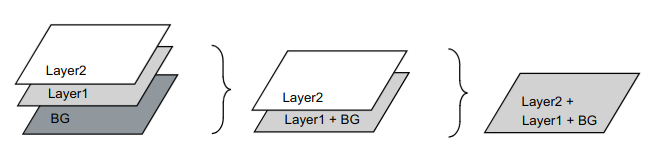
\includegraphics[width=0.6\textwidth]{material/figures/LCD-TFT_Layers.png.png}
    \caption{Zusammenfügen von zwei Layern \cite{rm0486}}
    \label{fig:lcd-tft-layers}
\end{figure}

Layer 1 bildet die Hintergrundebene und zeigt das von Pipe 1 erzeugte Kamerabild mit einer Auflösung von 800 × 480 Pixeln im RGB888-Format. Auf dieser Ebene werden außerdem die Region of Interest und die erkannten Handlandmarks in das jeweilige Kamerabild eingezeichnet. Layer 2 dient als Vordergrundebene für die grafische Benutzeroberfläche. Sie verwendet das ARGB4444-Format und unterstützt dadurch eine pixelweise Transparenz. Transparente Bereiche geben das darunterliegende Kamerabild frei, während Bedienelemente, Texte und Statusinformationen über diesem dargestellt werden können.

Die Abbildung veranschaulicht die Zusammensetzung der Displayausgabe. Zunächst wird Layer 1 über dem konfigurierten LTDC-Hintergrund dargestellt. Da Layer 1 das vollständige Display im RGB888-Format abdeckt, bildet er im regulären Betrieb den sichtbaren Hintergrund. Anschließend wird Layer 2 unter Berücksichtigung der im ARGB4444-Format enthaltenen Alphawerte darübergelegt. Transparente Bereiche von Layer 2 lassen das Kamerabild von Layer 1 sichtbar, während nicht transparente Bereiche die Elemente der Benutzeroberfläche darstellen. Das Ergebnis beider Ebenen wird anschließend als gemeinsames Bild an das Display ausgegeben. Die genaue Gestaltung und Aktualisierung der Benutzeroberfläche wird in Abschnitt~\ref{sec:visualisierung} beschrieben.

\section{Ablaufsteuerung und Software Scheduler}\label{sec:scheduler}

\subsection{Architektur-Übersicht}\label{sub:scheduler-architektur}
Mit der zunehmenden Komplexität einzelner Komponenten verlängert sich die Laufzeit dieser. Dies führt bei sequenzieller Ausführung zu dem Problem, dass Komponenten, die in einer bestimmten Frequenz ausgeführt werden müssen, nicht mehr rechtzeitig bedient werden können. Ein Beispiel hierfür ist das Display, das bei zu langsamer Zykluszeit nicht mehr interaktionsfähig bleibt, während beispielsweise die Kamera-Erfassung oder Sensorabfragen deutlich mehr Rechenzeit beanspruchen. Eine rein sequenzielle Schleife (super-loop, vgl.\ Abschnitt~\ref{sub:bare-metal}) kann diese unterschiedlichen Anforderungen nicht mehr befriedigen.

Als Lösung wurde ein prioritätsbasierter preemptiver Scheduler implementiert, der als Nicht-RTOS-Lösung auf dem ARM Cortex-M55 direct auf dem bare-metal läuft. Der Scheduler verwaltet maximal 9 Tasks, wobei Slot 8 fest dem Idle-Task zugewiesen ist, der im WFI-Zustand (Wait For Interrupt) verharrt und bei Bedarf Statistiken ausgibt.

Zeitgeber (Tick-Source): Als Zeitsystem dient TIM7 mit einer Periode von 1 ms, konfiguriert über APB1 mit 200 MHz Taktfrequenz. Der Timer generiert im \texttt{TIM7\_IRQHandler} einen Tick, der den System-Tick-Zaehler (\texttt{\_sys\_tick\_ms}) erhöt und bei abgelaufener Periode die jeweiligen Tasks in den TaskReady-Zustand ueberführt, gefolgt von einer PendSV-Anforderung zur Kontextwahl.

Kontextmodell: Pro Task wird der vollstaendige ARM-Kontext gespeichert. Der Scheduler nutzt den PSP (Process Stack Pointer) im Thread-Modus, wobei die FPU-Kontextspeicherung mittels lazy-stacking (ASPEN + LSPEN) erfolgt. Der zu speichernde Stack-Frame umfasst 32 Words: die FPU callee-saved Register S16–S31 (16 Words), die Core callee-saved Register R4–R11 (8 Words) sowie den 8-Word Hardware Exception Frame (R0–R3, R12, LR, PC, xPSR).

Stack-Management: Tasks erhalten einen variablen Stack, der aus einem statischen Bump-Allocator Pool mit 8192 Words (32 KB) alloziert wird. Die Stack-Grösse pro Task ist konfigurierbar (min. 144 Words, max. 2048 Words). Jeder Stack wird mit einem Canary-Muster (0xA5A5A5A5) gefüllt, um Stack-Overflows näher betrachten zu können. Der untere Stack-Schutz erfolgt über PSPLIM (Process Stack Limit Register), wobei die Guard-Zone 25\% der Stack-Groesse (64–512 Bytes) plus 32 Bytes Exception-Frame-Marge beträgt. Da der Bump-Allocator keine Deallocation unterstuetzt, wird bei einem Re-Add mit grösserer Stackanforderung der alte Block aufgegeben und ein neuer aus dem Pool allokiert.

Preemption: Tasks können durchhöherpriorisierte Tasks unterbrochen werden. Die Prioritäten reichen von 0 (höchste) bis 0xFF (niedrigste, Idle-Task). Die Kontextwahl erfolgt über PendSV (Pending supervisor call) mit der niedrigsten Interruptpriorität (0xFF), sodass alle anderen Interrupts zuerst abgearbeitet werden. Die Selektion des nächsten Tasks erfolgt mittels Round-Robin mit Prioritätssuche: Es wird ab dem aktuellen Task-Index zirkulär gesucht und der höchstpriorisierte bereite Task ausgewählt.

\subsection{Task-Lebenszyklus (State machine)}\label{sub:task-lebenszyklus}

\begin{figure}[H]
    \centering
    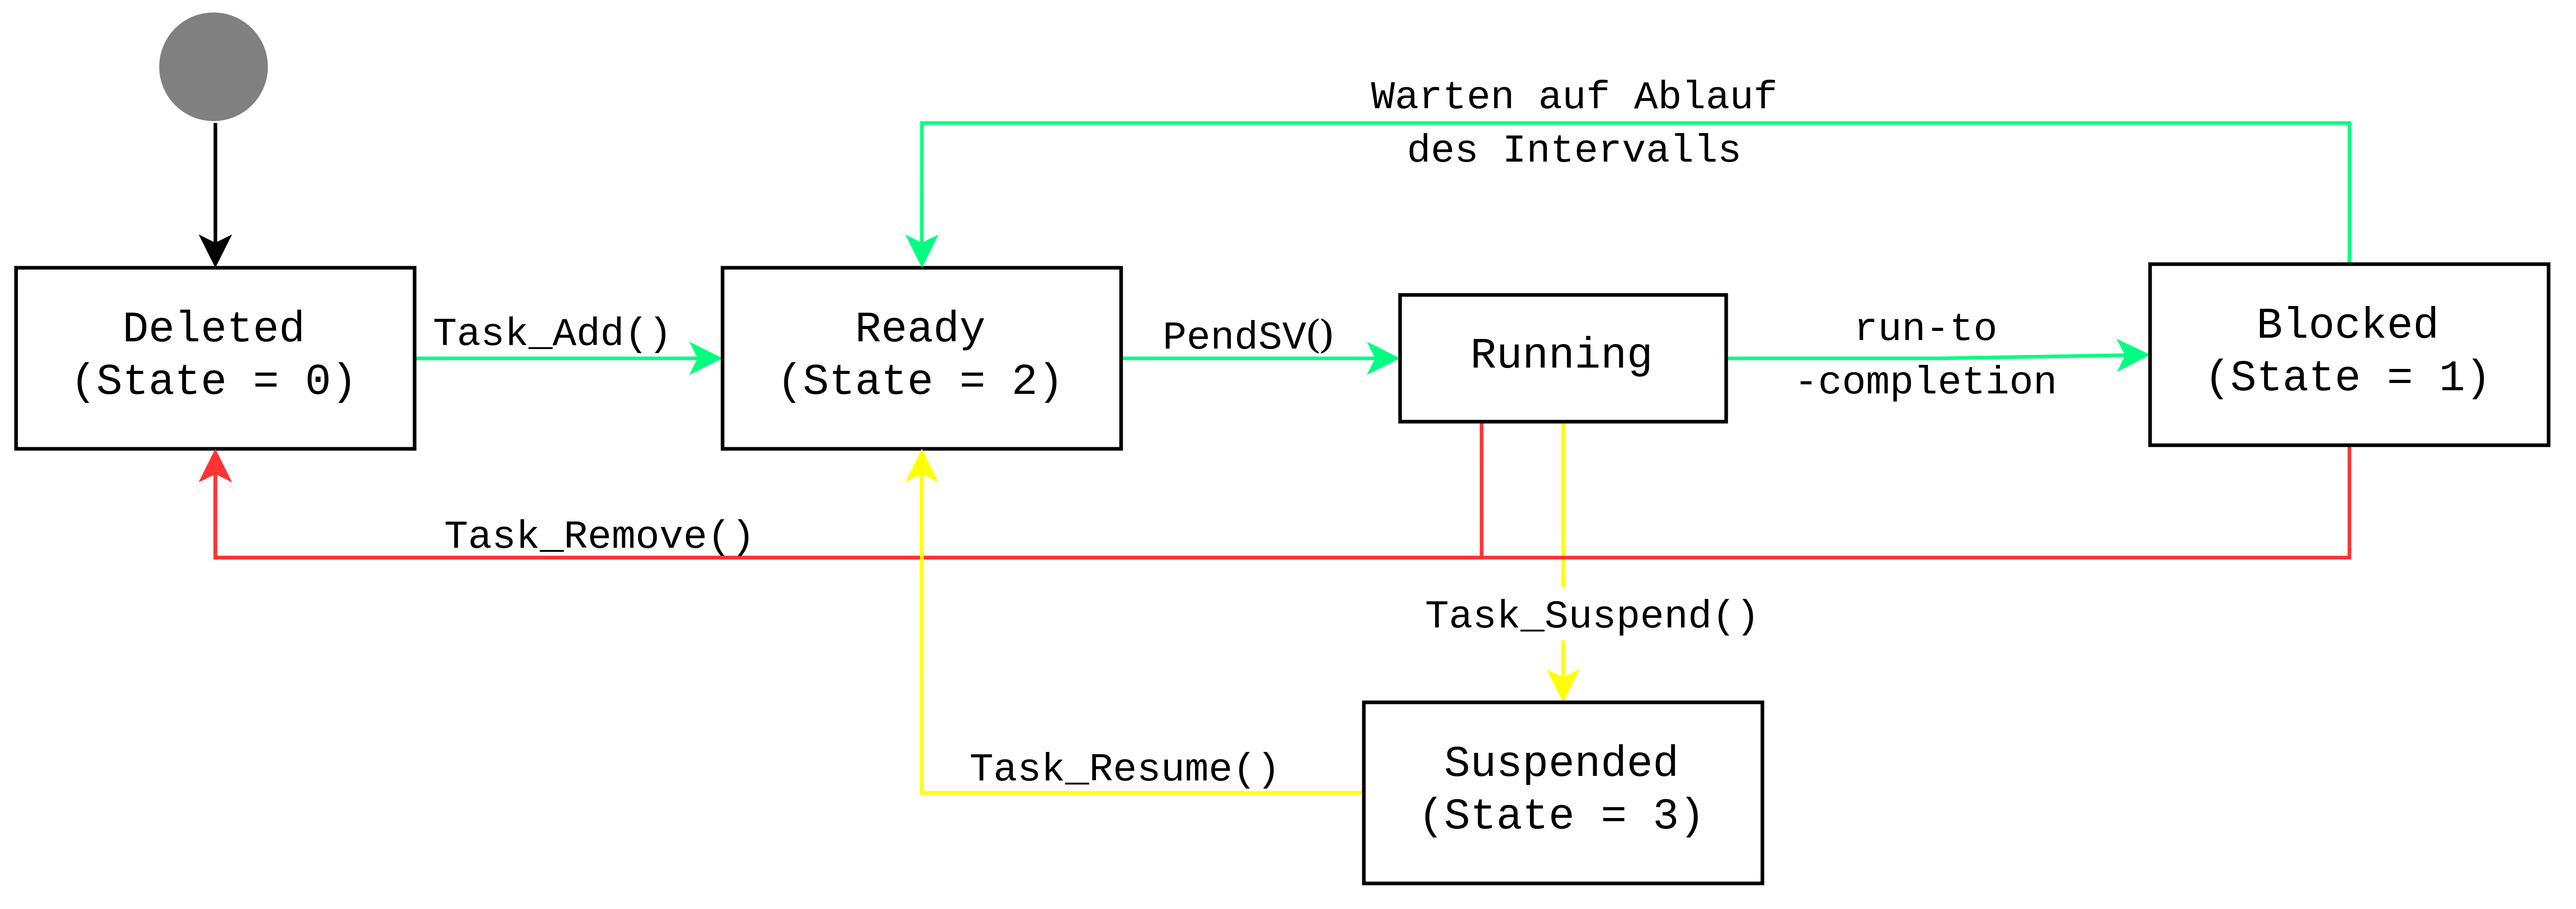
\includegraphics[width=1\linewidth]{material//figures/Task-States.drawio.png}
    \caption{Task-States des Schedulers}
    \label{fig:task-states}
\end{figure}

Ein Task hat vier Zustände:
\begin{itemize}
    \item \texttt{Deleted}: Task wartet auf Zuweisung eines Prozesses
    \item \texttt{Ready}: Task kann Ausgeführt werden. Wartet auf Scheduler Auswahl.
    \item \texttt{Blocked}: Task warted auf den Ablauf seiner Periode
    \item \texttt{Suspended}: Task wird an der gehindert Ausgeführt zu werden bis dieser weitergeführt werden kann. DMA2D pausiert Task bis die Speicheroperation erfolgt ist.
\end{itemize}

\ref{fig:task-states} stellt die Übergänge zwischen Zuständen dar.

\subsection{Interrupt-Hierrarchie \& Context Switching}\label{sub:interrupt-hierarchie}

Die Kontextwaehlerung ist der Kernmechanismus des Schedulers und erfolgt auf ARM Cortex-M55 auf drei Ebenen: dem anfänglichen Bootstrap des ersten Tasks, der periodischen Tick-gesteuerten Aktivierung via TIM7\_IRQHandler, und der eigentlichen Contextwaehlerung via PendSV\_Handler

\newpage

\subsubsection{Anfänglicher Context-Start (Bootstrapping)}\label{ssub:bootstrap}
Der Start des ersten Tasks erfolgt nicht ueber PendSV, sondern ueber einen SVC-Aufruf (Supervisor Call). Der Ablauf in \texttt{SCHEDULER\_Tasks\_run()} ist wie folgt

\begin{lstlisting}[language=bash, numbers=none, caption={Bootstrap Prozess}, label={lst:bootstrap}]
SCHEDULER_Tasks_run()
  |- IRQs deaktivieren (__disable_irq)
  |- Idle-Task registrieren (Slot 8, WFI-Loop)
  |- NVIC-Prioritaeten konfigurieren:
  |    SVCall  -> 0x00 (hoechste, fuer Bootstrap)
  |    TIM7    -> 0x80 (Scheduler-Tick)
  |    PendSV  -> 0xFF (niedrigste, Context-Switch)
  |- FPU lazy-stacking aktivieren (ASPEN + LSPEN)
  |- _Task_SelectNext() -> waehlt ersten bereiten Task
  |- Fault-Handler aktivieren (Hard/Mem/Bus/Usage)
  |- IRQs aktivieren (__enable_irq)
  \- SVC #0 ausführen des SVC_Handler
                |
                |
   SVC_Handler (naked, Assembler):
    1. _task_current laden (Slot-Index des ersten Tasks)
    2. TCB-Adresse berechnen: _tasks + (index × 28 Bytes)
    3. PSPLIM aus _task_psplims laden und setzen (Stack-Guard)
    4. saved_sp aus TCB laden -> PSP setzen
       (Zeigt auf den initialisierten Exception-Frame)
    5. R4-R11 vom Stack wiederherstellen
    6. PSP setzen
    7. CONTROL Register setzen:
       - SPSEL = 1 (PSP im Thread-Modus)
       - nPRIV = 0 (unprivileged - Task läuft im User-Mode)
    8. _StartTick() aufrufen:
       - TIM7 NVIC pending löschen
       - TIM7 NVIC enable
       - TIMER_Start(TIM7)
       - _scheduler_running = 1
    9. bx lr -> Sprung zur Task-Funktion (PC aus Exception-Frame)
\end{lstlisting}

\subsubsection{Periodische Aktivierung (Tim7\_IRQhandler)}\label{ssub:tim7-irq}
Alle 1ms löst der TIM7-Interrupt aus und steuert den Scheduling-Ablauf.
Jeder registrierte Task welcher nicht \texttt{TaskDeleted} oder \texttt{TaskSuspended} ist wird auf Ablauf des Ausführungs Intervalls geprüft. Tasks dessen Intervalle abgelaufen sind werden in \texttt{TaskReady} zustand versetzt. Damit der Task auswahl Algorithmus diese Auswählen kann. Im Anschluss wird die PendSV Ausführung angefordert.

PendSV wird nicht sofort ausgeführt, sondern läuft erst, wenn alle anderen ISRs abgearbeitet sind.

\subsubsection{Preemptiver Context-Switch (PendSV\_Handler)}\label{ssub:pendsv-handler}

Die eigentliche Kontextwahl erfolgt im \texttt{PendSV\_Handler}in reiner Assembler-Implementierung. PendSV hat die niedrigste NVIC-Priorität (0xFF), wird also erst nach Abschluss aller anderen Interrupts ausgeführt.

\begin{lstlisting}[language=bash, numbers=none, caption={PendSV\_Handler() in Hochsprache}, label={lst:pendsv-handler}]
PendSV\_Handler:
    1. IRQs deaktivieren (cpsid i) -> Verhindert Race-Condition während Context-Save
    2. Aktuellen PSP lesen (mrs r0, psp)
    3. Callee-Saved Register sichern:                  
       -> R4-R11 werden auf den aktuellen Task-Stack abgelegt
    4. FPU-Kontext sichern (bedingt):         
       -> Wenn EXC_RETURN Bit 4 = 0 wurde FPU benutzt:        
         S16-S31 werden ebenfalls gespeichert (16 Words)      
       -> Wenn Bit 4 = 1: kein FPU-Frame, Speicher gespart    
    5. Stack-Pointer in TCB sichern:                          
       TCB->saved_sp = r0                                     
       TCB->saved_exc_return = lr                             
    6. _Task_SelectNext() aufrufen (C-Funktion):              
       |- Scannt alle Tasks (Round-Robin ab _task_current+1)
       |- Waehlt hoechstpriorisierten TaskReady-Task
       |- Falls keiner bereit: IDLE_TASK (Slot 8)
       |- Aktualisiert CPU-Zyklen-Statistiken:
            - Vorherigen Task: total_cycles += active_cycles
            - Preemption-Zaehler erhoehen (falls Taskwechsel)  
            - Naechsten Task: invocations++, start_cycle setzen
       \- Gibt Index des naechsten Tasks zurueck
    7. _task_current = neuer Index
    8. Neuen TCB laden
    9. PSPLIM für neuen Task setzen:                     
       -> isb (Instruction Synchronization Barrier)
    10. Stack-Pointer vom neuen Stack wiederherstellen
    11. EXC_RETURN laden                                       
    12. FPU-Kontext wiederherstellen (bedingt):                                
       -> S16-S31 nur wenn FPU beim letzten Speichern benutzt
    13. Core-Register wiederherstellen:
        -> R4-R11 werden vom neuen Stack geladen
    14. PSP auf neuen Stack setzen
    15. IRQs aktivieren
    16. bx lr                                                  
       -> EXC_RETURN fuehrt zur Task-Rueckkehr:
            - Thread-Modus
            - PSP als Stack-Pointer
            - Stack-Frame automatisch popped (R0-R3,R12,LR,PC)
            - CPU springt zu PC (naechste Instruktion des Tasks)

\end{lstlisting}

\newpage

\subsection{Task-Selektion}\label{sub:task-selektion}

\begin{lstlisting}[language=pseudocode, numbers=none, caption={Selection of the next task to execute}, label={lst:task-select}]
Task_SelectNext():
    start = (_task_current + 1) mod IDLE_INDEX

    best = -1
    best_prio = 0xFF

    For n = 0 to (MAX_TASKS - 2):
        i = (start + n) mod IDLE_INDEX
        If (tasks[i].state == TaskReady):
            If (tasks[i].priority < best_prio):
                best = i
                best_prio = tasks[i].priority

    If best == -1:
        best = IDLE_TASK_INDEX  // Slot 8

    Update Statistics
    Return best
\end{lstlisting}

Bei gleicher Priorität entscheidet die Reihenfolge der Slot-Indizes (implizierter Round-Robin). Der Algorithmus scannt zirkulär ab dem nächsten Slot und wählt den Task mit der niedrigsten Prioritätszahl (0 = höchste).

\subsection{Fault handling}\label{sub:fault-handling}

Während der Ausführung der Tasks können sogenannte \emph{Faults} (Ausnahmezustaende) auftreten, die vom Cortex-M55-Prozessor erkannt und an den registrierten Fault-Handler weitergeleitet werden. Der Cortex-M55 unterscheidet zwischen mehreren Fault-Klassen (UsageFault, BusFault, MemManage Fault und HardFault | Abschnitt~\ref{sub:bare-metal}). Von den dort beschriebenen Auslösern ist in dieser Konfiguration insbesondere anzumerken, dass keine Memory Protection Unit (MPU) aktiv ist. Der MemManage-Fault wird daher hauptsächlich durch Eskalation aus anderen Fault-Typen oder durch Speicherzugriffe auf ungültige Adressen (z.\,B.\ Null-Pointer-Dereferenzierung) ausgelöst.

Diese Faults werden durch den Scheduler abgefangen. Dazu registriert der Scheduler in \texttt{SCHEDULER\_\allowbreak Tasks\_run()} die entsprechenden Fault-Handler (\texttt{HardFault\_Handler}, \linebreak \texttt{UsageFault\_Handler}, \texttt{Bus\allowbreak Fault\_Handler},  \texttt{MemManage\_Handler}) als naked-Assemble- \linebreak Funktionen, die den aktiven \allowbreak Stack-Frame (MSP oder PSP) ermitteln und an die C-Funktion \texttt{\_FaultHandler\_C()} übergeben. Der Handler erfasst den vollstaendigen diagnostischen Zustand des Systems, einschliesslich aller SCB-Register (\texttt{CFSR}, \texttt{HFSR}, \texttt{MMFAR}, \texttt{BFAR}), der Stack-Pointer (\texttt{MSP}, \texttt{PSP}, \texttt{PSPLIM}), des \texttt{CONTROL}-Registers, des \texttt{EXC\_RETURN}-Wertes sowie der gesicherten Register \texttt{R0--R3}, \texttt{R12}, \texttt{LR}, \texttt{PC} und \texttt{xPSR} und übertraegt diese Information per USART als Diagnoseausgabe. Anschliessend wird das Programm mittels Breakpoint-Befehl (\texttt{\_\_BKPT(0)}) für den Debugging-Prozess angehalten. Eine automatische Fehlerbehandlung oder Wiederherstellung des Betriebs findet nicht statt.

\subsection{CPU-Zyklen-Messung \& Statistik}\label{sub:cpu-statistik}

Um die Laufzeiteigenschaften der einzelnen Tasks zur Laufzeit bewerten zu können, implementiert der Scheduler eine hardwaregestützte CPU-Zyklen-Messung. Als Messquelle dient der DWT (Data Watchpoint and Trace) Modul des Cortex-M55-Prozessors, dessen Zykelzähler \texttt{DWT->CYCCNT} bei Systemtaktfrequenz (200\,MHz) hochauflösend incremental zählt. Die Aktivierung erfolgt in \texttt{SCHEDULER\_System\_init()} durch Setzen der \texttt{DEMCR\_TRCENA} und \linebreak \texttt{DWT\_CYCCNTENA} Bits.

\paragraph{Per-Task-Erfassung}
Für jeden Task werden in der Struktur \texttt{\_Task\_Stats\_TypeDef} folgende Metriken geführt:
\begin{itemize}
    \item \texttt{total\_cycles}: Summe der reinen Applikations-Zyklen abzüglich der in Interrupt-Kon-text verbrachten Zeit
    \item \texttt{total\_preempts}: Anzahl der Unterbrechungen durch höherpriorisierte Tasks
    \item \texttt{total\_invocations}: Gesamtzahl der Task-Aufrufe
    \item \texttt{min\_cycles} / \texttt{max\_cycles}: Minimaler und maximaler Zykelverbrauch pro Aufruf
\end{itemize}
Die Messung erfolgt bei jedem Context-Switch im \texttt{\_Task\_SelectNext()}: Der seit dem letzten Start vergangene Zeitraum wird ermittelt und von den im \texttt{\_task\_isr\_cycles}-Array kumulierten ISR-Zyklen subtrahiert. Das Ergebnis repräsentiert den reinen Applikationsanteil (\texttt{\%ACT}) des vorherigen Tasks.

\paragraph{ISR-Cycle-Tracking}
Um Interrupt-Zyklen sauber von Task-Zyklen zu trennen, muss jede Peripheral-ISR am Ein- und Ausgang die Funktionen \texttt{SCHEDULER\_ISR\_enter()} und \linebreak \texttt{SCHEDULER\_ISR\_exit()} aufrufen. Bei Einstieg wird der aktuelle \texttt{DWT->CYCCNT}-Wert gespeichert. Bei Ausgang wird die Differenz berechnet und dem unterbrochenen Task in \linebreak \texttt{\_task\_isr\_cycles} zugeordnet.

\paragraph{Ausgabe}
Alle 1000\,ms, getriggert durch den \texttt{TIM7\_IRQHandler}, wird \texttt{\_stats\_pending} gesetzt und im Idle-Task die Funktion \texttt{\_PrintStats()} aufgerufen. Diese erzeugt eine tabellarische Ausgabe mit den Spalten \texttt{Name}, \texttt{cycle} (Gesamt-Zyklen), \texttt{min}, \texttt{max}, \texttt{avg} (durchschnittliche Zyklen pro Invocation), \texttt{\%ACT} (Aktiv-Anteil in Prozent), \texttt{Prempt} (Preemption-Zaehler) und \texttt{Invoc} (Invocation-Anzahl). Zusätzlich werden der Gesamtanteil idle-Zeit, der ISR-Overhead und die CPU-Auslastung in Prozent ausgegeben. Die Statistik wird nach jedem Druckvorgang zurückgesetzt, sodass jeder Messzeitraum den Zeitraum zwischen zwei aufeinanderfolgenden Ausgaben repräsentiert.

\section{Integration der NPU und einheitliche KI-Schnittstelle}\label{sec:npu-integration}

Die Ausführung der drei neuronalen Netze erfolgt überwiegend auf dem im STM32N6570-DK integrierten Neural-ART Accelerator. Für dessen Verwendung müssen zunächst die zugehörigen Takt- und Speicherbereiche sowie die ATON-Laufzeitumgebung eingerichtet werden. Anschließend werden die drei konvertierten Netzwerkinstanzen für die Handdetektion, Landmark-Erkennung und Fingeralphabetklassifikation initialisiert.

Um die Middleware-spezifischen Aufrufe nicht unmittelbar in der Ablaufsteuerung verwenden zu müssen, wurde mit \texttt{simple\_ai} eine gemeinsame KI-Schnittstelle umgesetzt. Diese fasst die Initialisierung der KI-Komponenten zusammen, vereinheitlicht die Statusrückgaben und stellt Funktionen für die Ausführung der neuronalen Netze bereit.

\subsection{Initialisierung des Neural-ART Accelerators}\label{sub:npu-init}

Die Initialisierung der KI-Komponenten erfolgt zentral durch \texttt{AI\_Init()}. Die Funktion prüft zunächst, ob die Initialisierung bereits durchgeführt wurde. In diesem Fall wird unmittelbar \texttt{AI\_\allowbreak STATUS\_OK} zurückgegeben. Dadurch kann die Funktion mehrfach aufgerufen werden, ohne die Laufzeitumgebung und Netzwerkinstanzen erneut einzurichten. Zu Beginn werden die benötigten Takt- und Speicherbereiche aktiviert.

Innerhalb dieser Funktion wird außerdem die Konfiguration des NPU-Caches vorgenommen. Die anschließende Initialisierung des CacheAXI erfolgt über \texttt{HAL\_CACHEAXI\_Init()}. CacheAXI stellt die für die NPU erforderliche Cache-Infrastruktur bereit. Da die Initialisierung durch die von STMicroelectronics bereitgestellte HAL-Komponente erfolgt, bildet sie eine Ausnahme von der ansonsten überwiegend registerbasierten Treiberimplementierung. Schlägt dieser Schritt fehl, wird die Initialisierung mit \texttt{AI\_STATUS\_CACHEAXI\_ERROR} abgebrochen.  

Der verwendete \texttt{CACHEAXI-HAL}-Treiber erwartet für seine interne Zeitüberwachung die Funktion  \texttt{HAL\_GetTick()}. Da im Projekt keine separate HAL-Zeitbasis verwendet wird, wurde mit \texttt{ai\_hal\_adapter.c} ein kleiner Adapter umgesetzt. Die Funktion \texttt{HAL\_GetTick()} greift auf den bereits vorhandenen Millisekundenzähler des Software-Schedulers zurück. Dadurch kann der \texttt{CACHE\allowbreak AXI}-Treiber seine vorgesehenen Zeitüberwachungen verwenden, ohne zusätzlich den vollständigen HAL-Zeitbasismechanismus in das Projekt zu integrieren. 

Nach erfolgreicher Einrichtung der Hardware wird \texttt{LL\_ATON\_RT\_RuntimeInit()} aufgerufen. Diese Funktion initialisiert die ATON-Laufzeitumgebung, über die die konvertierten neuronalen Netze ausgeführt werden. Anschließend werden die drei Netzwerkinstanzen nacheinander initialisiert:

\begin{enumerate}
    \item Handdetektion über \texttt{PALM\_Init()}
    \item Landmark-Erkennung über \texttt{LANDMARK\_Init()}
    \item Fingeralphabetklassifikation über \texttt{FINGERALPHABET\_Init()}
\end{enumerate}

Jede Initialisierungsfunktion ermittelt die vom jeweiligen Netzwerk verwendeten Ein- und Ausgabepuffer und bereitet dessen internen Zustand vor. Gibt eine der Funktionen einen Fehlerstatus zurück, wird die weitere Initialisierung abgebrochen und der Status an die aufrufende Komponente weitergereicht. Erst nach erfolgreicher Initialisierung aller drei Modelle wird \texttt{ai\_initialized} gesetzt und \texttt{AI\_STATUS\_OK} zurückgegeben.

\subsection{Einheitliche KI-Schnittstelle}\label{sub:ki-schnittstelle}

Die von der ATON-Middleware bereitgestellten Funktionen sind an die Laufzeitumgebung und die jeweils erzeugten Netzwerkinstanzen gekoppelt. Um diese Abhängigkeiten nicht unmittelbar in die Ablaufsteuerung und die Vor- bzw. Nachverarbeitung zu übernehmen, wurde mit \texttt{simple\_ai} eine gemeinsame KI-Schnittstelle implementiert. Sie bündelt die allgemeinen Funktionen zur Initialisierung und Ausführung der neuronalen Netze und stellt einheitliche Statuswerte für alle Modellkomponenten bereit.

Für die Rückgabe von Fehlerzuständen wird der gemeinsame Aufzählungstyp \texttt{AI\_Status\_\allowbreak TypeDef} verwendet. Dadurch können die zentralen und modellspezifischen KI-Funktionen ihre Ergebnisse in einer einheitlichen Form an die aufrufenden Komponenten weitergeben. Die Ablaufsteuerung muss somit keine unterschiedlichen Fehlerdarstellungen der einzelnen Modelle auswerten.

\begin{longtable}{|p{0.4\textwidth}|p{0.5\textwidth}|}
    \hline
    \textbf{Statuswert} & \textbf{Bedeutung} \\
    \hline
    \endfirsthead
    \hline
    \textbf{Statuswert} & \textbf{Bedeutung} \\
    \hline
    \endhead
    \hline
    \multicolumn{2}{r}{\texttt{Fortsetzung auf nächster Seite}} \\
    \endfoot
    \caption{Einheitliche Statuswerte der KI-Komponenten}
    \label{tab:ki-statuswerte} \\
    \endlastfoot
    \texttt{AI\_STATUS\_OK}                & Die aufgerufene Funktion wurde erfolgreich ausgeführt. \\
    \hline
    \texttt{AI\_STATUS\_NOT\_INITIALIZED}  & Die benötigte KI-Komponente wurde noch nicht initialisiert. \\
    \hline
    \texttt{AI\_STATUS\_CACHEAXI\_ERROR}   & Bei der Einrichtung des CacheAXI ist ein Fehler aufgetreten. \\
    \hline
    \texttt{AI\_STATUS\_INVALID\_BUFFER}   & Ein benötigter Ein- oder Ausgabepuffer ist ungültig. \\
    \hline
    \texttt{AI\_STATUS\_PREPROCESS\_ERROR} & Die Vorverarbeitung der Eingabedaten ist fehlgeschlagen. \\
    \hline
    \texttt{AI\_STATUS\_POSTPROCESS\_ERROR}& Die Nachverarbeitung der Modellausgabe ist fehlgeschlagen. \\
    \hline
    \texttt{AI\_STATUS\_RUNTIME\_ERROR}    & Während der Ausführung eines Modells ist ein Fehler aufgetreten. \\
    \hline
\end{longtable}

Die eigentliche Ausführung einer Netzwerkinstanz wird durch \texttt{AI\_RuntimeRunNetwork()} gekapselt. Der Funktion wird ein Zeiger auf die jeweilige \texttt{NN\_Instance\_TypeDef} übergeben. Dadurch kann dieselbe Funktion für die Handdetektion, die Landmark-Erkennung und die Fingeralphabetklassifikation verwendet werden. Ist der übergebene Zeiger ungültig, wird die Ausführung unmittelbar abgebrochen. Intern ruft die Funktion wiederholt \texttt{LL\_ATON\_RT\_RunEpoch\allowbreak Block()} auf. Die ATON-Laufzeitumgebung verarbeitet das Netzwerk dabei abschnittsweise und liefert nach jedem Aufruf einen Status zurück. Mit \texttt{LL\_ATON\_RT\_WFE} wird signalisiert, dass zunächst auf ein Hardwareereignis gewartet werden muss. In diesem Fall erfolgt das Warten über \texttt{LL\_ATON\_OSAL\_WFE()}. Der Status \texttt{LL\_ATON\_RT\_NO\_WFE} zeigt dagegen an, dass die Verarbeitung ohne vorheriges Warten fortgesetzt werden kann. Die Aufrufe werden wiederholt, bis die Laufzeitumgebung einen abschließenden Status zurückgibt.

Die Funktion liefert nur dann \texttt{true}, wenn die Netzwerkausführung mit \texttt{LL\_ATON\_RT\_DONE} beendet wurde. Alle anderen abschließenden Zustände werden als fehlgeschlagene Ausführung behandelt und durch \texttt{false} signalisiert. Für die aufrufenden Modellkomponenten entsteht dadurch eine vereinfachte Schnittstelle, bei der die einzelnen ATON-Rückgabewerte nicht außerhalb von \texttt{simple\_ai} ausgewertet werden müssen.

Die modellspezifischen Komponenten kapseln darauf aufbauend die jeweiligen Netzwerkinstanzen sowie deren Ein- und Ausgabepuffer. Sie prüfen ihren Initialisierungszustand und die übergebenen Puffer, führen die Netzwerkinstanz über \texttt{AI\_RuntimeRunNetwork()} aus und übersetzen das Ergebnis in einen Wert des gemeinsamen Typs \texttt{AI\_Status\_TypeDef}. Die Vor- und Nachverarbeitung verbleibt hingegen in den jeweiligen Modellkomponenten, da sie sich zwischen Handdetektion, Landmark-Erkennung und Fingeralphabetklassifikation unterscheidet.

Damit bildet \texttt{simple\_ai} die gemeinsame Verbindung zwischen den erzeugten Netzwerkinstanzen und der übergeordneten Ablaufsteuerung. Middleware-spezifische Details der Netzwerkausführung bleiben innerhalb dieser Schnittstelle gekapselt, während die modellspezifischen Unterschiede weiterhin in den zugehörigen Komponenten behandelt werden.

\section{Vor- und Nachverarbeitungsschritte}\label{sec:vor-nachverarbeitung}

Die drei neuronalen Netze verwenden unterschiedliche Eingabedaten und liefern Ausgaben, die nicht unmittelbar durch das jeweils nachfolgende Modell verarbeitet werden können. Daher sind zwischen den einzelnen Inferenzschritten mehrere Vor- und Nachverarbeitungen erforderlich. Diese umfassen sowohl hardwaregestützte Operationen innerhalb der DCMIPP als auch durch den Hauptprozessor ausgeführte Transformationen der Bild- und Landmark-Daten.

\subsection{DCMIPP-gestützte Bildvorverarbeitung}\label{sub:dcmipp-vorverarbeitung}

Die Kamera überträgt die aufgenommenen Bilder als RAW-Bayer-Daten mit einer Auflösung von 2592x1944 Pixeln über die CSI-Schnittstelle. Da weder die Displayausgabe noch die neuronalen Netze diese Daten unmittelbar verarbeiten können, übernimmt die Digital Camera Interface Pixel Pipeline (DCMIPP) einen wesentlichen Teil der erforderlichen Bildvorverarbeitung. Die DCMIPP wandelt die RAW-Bayer-Daten zunächst in ein RGB-Bild um. Hierzu werden die Demosaikierung der RAW10-Bilddaten, die Farbkorrektur, die Belichtungsanpassung und die Gammakorrektur innerhalb der Bildpipeline durchgeführt \cite[S. 1815 ff.]{rm0486}. Das Ergebnis wird im RGB888-Format ausgegeben. Dadurch müssen diese rechenintensiven Verarbeitungsschritte nicht nachträglich durch den Hauptprozessor auf den bereits gespeicherten Kamerabildern ausgeführt werden.

Die verwendeten Parameterwerte wurden empirisch bestimmt. Hierzu wurden die entsprechenden DCMIPP-Register schrittweise angepasst und die Auswirkungen auf das ausgegebene Kamerabild visuell bewertet. Einstellungen, die unter den vorgesehenen Einsatzbedingungen eine geeignete Bilddarstellung ergaben, wurden anschließend in die feste Konfiguration der Bildpipeline übernommen.

Aus dem gemeinsamen Kameradatenstrom werden zwei getrennte Ausgabepfade erzeugt. Pipe 1 dient der Displayausgabe und stellt gleichzeitig das Ausgangsbild für die Landmark-Erkennung bereit. Pipe 2 erzeugt dagegen das Eingabebild für die Handdeteketion.

Für Pipe 1 wird das Sensorbild zunächst auf das Seitenverhältnis des Displays zugeschnitten. Der horizontale Bildbereich bleibt vollständig erhalten, während das Bild vertikal zentriert beschnitten wird. Der entstandene Ausschnitt wird anschließend durch die Downscaling-Einheit der DCMIPP auf eine Auflösung von 800x480 Pixeln verkleinert und im RGB888-Format im externen PSRAM abgelegt. Die von Pipe 1 erzeugten Bilder werden über vier Hintergrundbildpuffer verwaltet. Die DCMIPP schreibt jeweils in den für die Aufnahme vorgesehenen Puffer, während weitere Puffer für die Displayausgabe, die KI-Verarbeitung und das Einzeichnen der Handregion beziehungsweise der Landmarks verwendet werden. Nach Abschluss eines Bildes wird die Zieladresse der DCMIPP auf den nächsten Aufnahmepuffer umgeschaltet.

Pipe 2 verarbeitet den vollständigen Sensorbereich und erzeugt das Eingabebild für die Handdetektion. Da deren Eingangsauflösung mit 192x192 Pixeln deutlich unterhalb der Sensorauflösung liegt, wird das Bild vor der eigentlichen Skalierung horizontal und vertikal dezimiert. Dadurch reduziert sich die Auflösung zunächst von 2592x1944 auf 1296x972 Pixel. Anschließend übernimmt der DCMIPP-Downsizer die Skalierung auf 192x192 Pixel. Da vor der Skalierung kein quadratischer Bildausschnitt gebildet wird, wird das Seitenverhältnis des vollständigen Sensorbildes dabei an die quadratische Modelleingabe angepasst. Auch dieser Ausgabepfad verwendet das RGB888-Format. Für Pipe 2 wird der Double-Buffer-Modus der DCMIPP verwendet. Die erzeugten Bilder werden abwechselnd in zwei Eingabebildpuffern gespeichert. Während die DCMIPP einen Puffer mit einem neuen Bild beschreibt, kann der zuvor fertiggestellte Puffer für die Handdetektion verwendet werden. Der jeweils abgeschlossene Puffer wird über den Frame-Callback bestimmt und für die weitere Verarbeitung markiert.

\begin{longtable}{|p{0.18\textwidth}|p{0.125\textwidth}|p{0.125\textwidth}|p{0.45\textwidth}|}
    \hline
    \textbf{Parameter} & \textbf{Pipe 1} & \textbf{Pipe 2} & \textbf{Begründung} \\
    \hline
    \endfirsthead
    \hline
    \textbf{Parameter} & \textbf{Pipe 1} & \textbf{Pipe 2} & \textbf{Begründung} \\
    \hline
    \endhead
    \hline
    \multicolumn{4}{r}{\texttt{Fortsetzung auf nächster Seite}} \\
    \endfoot
    \caption{Konfigurationsparameter der DCMIPP-Bildpfade}
    \label{tab:dcmipp-konfig} \\
    \endlastfoot
    \texttt{output\_width} / \texttt{output\_height} & 800x480 & 192x192 & Entsprechen der Displayauflösung, bzw. Eingangsgröße der Handdetektion. \\
    \hline
    \texttt{output\_format} & RGB888 & RGB888 & Display und KI-Vorverarbeitung arbeiten mit drei Farbkanälen und jeweils 8 Bit pro Kanal. \\
    \hline
    \texttt{output\_bpp} & 3 & 3 & RGB888 benötigt drei Byte pro Pixel (für jeden Kanal 8 Bit). Der Wert wird unter anderem zur Berechnung des Speicher-Pitchs verwendet. \\
    \hline
    \texttt{enable\_crop} & aktiviert & aktiviert & Pipe 1 benötigt einen Zuschnitt auf das Seitenverhältnis des Displays. Pipe 2 verarbeitet den vollständigen Sensorbereich. \\
    \hline
    \texttt{crop\_x} & 0 & 0 & Horizontal wird kein Bereich abgeschnitten. \\
    \hline
    \texttt{crop\_y} & Zentriert vertikaler Zuschnitt & 0 & Pipe 1 entfernt oben und unten Bildbereiche, um das Sensorformat ohne Verzerrung an 800x480 anzupassen. Pipe 2 verwendet das vollständige Bild. \\
    \hline
    \texttt{crop\_width} & 2592 & 2592 & Die vollständige Sensorbreite wird verwendet. \\
    \hline
    \texttt{crop\_height} & 1555 & 1944 & Pipe 1 erhält das Displayseitenverhältnis 5:3. Pipe 2 behält die vollständige Sensorhöhe. \\
    \hline
    \texttt{enable\_\linebreak downsize} & aktiviert & aktiviert & Beide Ausgaben sind wesentlich kleiner als das Sensorbild. \\
    \hline
    \texttt{enable\_\linebreak decimate} & deaktiviert & aktiviert & Nur Pipe 2 benötigt vor dem Downscaling eine zusätzliche Halbierung. \\
    \hline
    \texttt{decimate\_h} / \texttt{decimate\_v} & -- & 1, 1 & Die Auflösung wird horizontal und vertikal jeweils durch zwei geteilt. \\
    \hline
    \texttt{enable\_swap} & deaktiviert & deaktiviert & Die Farbkanäle sind bereits korrekt. Ein Swap ist nicht notwendig. \\
    \hline
    \texttt{enable\_gamma} & aktiviert & aktiviert & Die Gammakorrektur verbessert die Helligkeitsdarstellung. \\
    \hline
    \texttt{enable\_dbm} & deaktiviert & aktiviert & Pipe 1 verwendet eine softwareseitige Rotation von vier Bildpuffern, da die Anwendung mehr als zwei Puffer benötigt. Pipe 2 verwendet zwei hardwareseitig wechselnde Eingabepuffer. \\
    \hline
\end{longtable}

Durch die hardwaregestützte Vorverarbeitung werden nur die tatsächlich benötigten Bildauflösungen in den externen Speicher geschrieben. Dies reduziert sowohl den Speicherbedarf als auch die vom Hauptprozessor zu verarbeitende Datenmenge. Die weiteren auf der CPU ausgeführten Vor- und Nachverarbeitungsschritte können dadurch unmittelbar auf den bereits aufbereiteten RGB888-Bilddaten arbeiten.

\subsection{Nachverarbeitung der Handdetektion}\label{sub:nachverarbeitung-palm}
\subsubsection{Ankerbasierte Modellausgabe}\label{ssub:ankerbasierung}

Das Modell zur Handdetektion verwendet ein ankerbasiertes Detektionsverfahren. Hierfür sind in der Ankertabelle \texttt{pd\_anchors} insgesamt 2016 Ankerpositionen definiert. Diese repräsentieren unterschiedliche Positionen und Größen möglicher Handregionen innerhalb des 192x192 Pixel großen Eingabebildes. Für jeden Anker gibt das Modell einen Konfidenzwert sowie mehrere Regressionswerte aus. Der Konfidenzwert beschreibt, wie wahrscheinlich sich im Bereich des jeweiligen Ankers eine Hand befindet. Die Regressionswerte enthalten die Abweichungen zwischen dem Anker und der vorhergesagten Handregion sowie die Positionen der zugehörigen Schlüsselpunkte \cite{zhangMediaPipeHandsOndevice2020}.

Die Anker bilden damit ein festes Suchraster über dem Eingabebild. Das Modell muss die Position und Ausdehnung einer Hand nicht vollständig unabhängig bestimmen, sondern sagt für jeden Anker die räumlichen Abweichungen zur tatsächlichen Handregion voraus. Da mehrere benachbarte Anker auf dieselbe Hand reagieren können, entstehen üblicherweise mehrere ähnliche Erkennungskandidaten, die in der anschließenden Nachverarbeitung bereinigt werden müssen.

\subsubsection{Auswahl und Filterung der Erkennungskandidaten}\label{ssub:kandidaten-filterung}
Für jeden der 2016 Anker wird zunächst geprüft, ob der ausgegebene Konfidenzwert den festgelegten Schwellwert erreicht. Die Konfidenzwerte liegen als Logits vor und müssen für die weitere Bewertung durch eine Sigmoidfunktion in einen Wahrscheinlichkeitswert zwischen 0 und 1 überführt werden \cite{sharmaACTIVATIONFUNCTIONSNEURAL2020}:
$$ \sigma(x) = \frac{1}{1 + \mathrm{e}^{-x}} $$
Eine direkte Berechnung würde die Exponentialfunktion \texttt{expf()} erfordern. Da die verwendete Floating Point Unit keine Exponentialfunktion als direkte Hardwareoperation bereitstellt, müsste diese softwareseitig berechnet werden. Zur Verringerung des Rechenaufwands wird die Sigmoidfunktion daher durch die folgende rationale Funktion approximiert:
$$\hat{\sigma}(x)=\frac{0{,}5+0{,}25x}{1-0{,}25x+0{,}125x^2}$$
Um die Sigmoidapproximation nicht für alle 2016 Anker ausführen zu müssen, wird der festgelegte Konfidenzschwellwert zunächst in den Logit-Raum überführt \cite[S. 340 ff.]{athavaleVerifyingGlobalTwoSafety2024}:
$$ t_{\mathrm{Logit}} = \ln\left(\frac{t}{1-t}\right) $$
Die vom Modell ausgegebenen Logits können dadurch unmittelbar mit dem berechneten Logit-Schwellwert verglichen werden. Nur Kandidaten, die diesen Schwellwert erreichen oder überschreiten, werden vollständig dekodiert und mithilfe der approximierten Sigmoidfunktion in einen Wahrscheinlichkeitswert umgerechnet. Anschließend werden die Regressionswerte der verbleibenden Kandidaten unter Berücksichtigung der jeweils zugehörigen Ankerposition dekodiert. Dabei werden der Mittelpunkt, die Breite und Höhe der vorhergesagten Handregion sowie die vom Modell ausgegebenen Schlüsselpunkte bestimmt. Die berechneten Koordinaten und Abmessungen werden auf die Größe des Modelleingangs normiert. Kandidaten mit einer ungültigen Breite oder Höhe sowie nicht endlichen Zahlenwerten werden verworfen.

Um den Speicherbedarf und den Rechenaufwand der weiteren Verarbeitung zu begrenzen, werden höchstens 20 Erkennungskandidaten zwischengespeichert. Diese Obergrenze wird durch die Konstante \texttt{PALM\_PP\_MAX\_CANDIDATES} festgelegt. Solange die maximale Anzahl noch nicht erreicht ist, wird jeder gültige Kandidat übernommen. Ist der Kandidatenspeicher bereits vollständig belegt, wird zunächst der Kandidat mit der geringsten Wahrscheinlichkeit ermittelt. Dieser wird nur dann ersetzt, wenn der neue Kandidat eine höhere Wahrscheinlichkeit aufweist. Auf diese Weise werden aus den Ergebnissen der 2016 Ankerpositionen ausschließlich die 20 wahrscheinlichsten Kandidaten für die weitere Verarbeitung berücksichtigt.

Die ausgewählten Kandidaten werden anschließend absteigend nach ihrer Wahrscheinlichkeit sortiert. Da mehrere benachbarte Anker auf dieselbe Hand reagieren können, entstehen häufig mehrere stark überlappende Handregionen. Zur Entfernung dieser Mehrfacherkennungen wird eine Non-Maximum Suppression (NMS) durchgeführt \cite{bodlaSoftNMSImprovingObject2017}. Hierzu wird jeder Kandidat mit den bereits übernommenen Handregionen verglichen. Als Maß für ihre räumliche Überschneidung dient die Intersection over Union (IoU). Sie beschreibt das Verhältnis zwischen der Schnittfläche und der Vereinigungsfläche zweier Begrenzungsrahmen \cite[S. 3]{rezatofighiGeneralizedIntersectionUnion2019}:
$$ \operatorname{IoU}(A,B) =\frac{\left|A \cap B\right|} {\left|A \cup B\right|} $$
Die Kandidaten werden in absteigender Reihenfolge ihrer Wahrscheinlichkeit verarbeitet. Erreicht oder überschreitet die IoU eines Kandidaten mit einer bereits übernommenen Handregion den festgelegten Schwellwert, wird der Kandidat verworfen. Dadurch bleibt von mehreren stark überlappenden Erkennungen in der Regel nur der Kandidat mit der höchsten Wahrscheinlichkeit erhalten. Nach Abschluss der Non-Maximum Suppression wird der stärkste verbleibende Kandidat als Ergebnis der Handdetektion übernommen. Das Ergebnis enthält die Wahrscheinlichkeit, den Mittelpunkt und die Abmessungen der erkannten Handregion, die zugehörigen Schlüsselpunkte sowie den verwendeten Ankerindex.

Um kurzzeitige Fehldetektionen und einzelne Aussetzer zu reduzieren, wird das Ergebnis zusätzlich über mehrere Ausführungen hinweg gefiltert. Eine Hand gilt erst dann als bestätigt, wenn in zwei aufeinanderfolgenden Auswertungen eine gültige Detektion vorliegt. Bei einer ungültigen Detektion wird der positive Zähler zurückgesetzt. Umgekehrt wird der erkannte Zustand erst aufgehoben, wenn in drei aufeinanderfolgenden Auswertungen keine gültige Handdetektion vorliegt. Einzelne Aussetzer führen dadurch nicht unmittelbar zum Verlust der erkannten Handregion.

\subsubsection{Erzeugung der initialen Region of Interest}\label{ssub:initiale-roi}

Aus der bestätigten Handdetektion wird die initiale Region of Interest für das Handlandmark-Modell erzeugt. Die Handdetektion wird auf dem von Pipe 2 bereitgestellten Bild ausgeführt, während der Eingabeausschnitt für das Landmark-Modell aus dem Displaybild von Pipe 1 entnommen wird. Aufgrund der unterschiedlichen Auflösungen und Bildausschnitte müssen die normierten Koordinaten der Handdetektion zunächst in das Koordinatensystem von Pipe 1 transformiert werden. In horizontaler Richtung bilden beide Bildpfade die vollständige Sensorbreite ab. Die horizontale Position und Breite können deshalb unmittelbar mit der Breite des Displaybildes skaliert werden. Pipe 1 verwendet jedoch einen vertikal zentrierten Ausschnitt des Sensorbildes. Bei der Transformation der vertikalen Koordinaten müssen daher zusätzlich die Höhe und der Offset dieses Ausschnitts berücksichtigt werden. Diese Koordinatentransformation wurde aus der Konfiguration der beiden DCMIPP-Pipelines abgeleitet.

Neben der Begrenzungsbox stellt das Modell mehrere Schlüsselpunkte der Hand bereit. In Anlehnung an die MediaPipe-Referenzimplementierung werden zwei dieser Punkte zur Bestimmung der Handorientierung verwendet. Der zwischen ihnen gebildete Richtungsvektor wird auf einen Zielwinkel von 90° und damit auf die vertikale Achse der Region ausgerichtet \cite{srccode_mediapipe}. Da die $y$-Achse in Bildkoordinaten nach unten zeigt, wird ihre Richtungsdifferenz mit umgekehrtem Vorzeichen berücksichtigt. Der Rotationswinkel ergibt sich damit zu:
$$\alpha = \frac{\pi}{2} - \operatorname{atan2}(-\Delta y,\Delta x)$$
Dabei bezeichnen $\Delta x$  und $\Delta y$ die Koordinatendifferenzen zwischen den verwendeten Schlüsselpunkten. Der berechnete Winkel wird anschließend auf den Bereich von $-\pi$ bis $\pi$ normiert. Kann aufgrund ungültiger Koordinaten kein eindeutiger Winkel bestimmt werden, wird für die Region eine Rotation von 0 verwendet.

Da die Begrenzungsbox der Handdetektion hauptsächlich die Handfläche umfasst, wird sie für die Landmark-Erkennung erweitert. Ihr Mittelpunkt wird entlang der rotierten lokalen Vertikalachse um die Hälfte der ursprünglichen Höhe in Richtung der Finger verschoben. Anschließend wird die längere Seite der Begrenzungsbox bestimmt und mit dem Faktor 2,6 skaliert. Der berechnete Wert wird für die Breite und Höhe verwendet, sodass eine quadratische Region entsteht. Die Verschiebung, Skalierung und quadratische Ausrichtung orientieren sich ebenfalls an der MediaPipe-Referenzimplementierung \cite{srccode_mediapipe}. Aus dem Mittelpunkt, der Seitenlänge und dem Rotationswinkel werden abschließend die vier Eckpunkte der Region berechnet. Die so erzeugte Region bildet die Grundlage für den 224x224 Pixel großen Eingabeausschnitt des Handlandmark-Modells. Dessen Erzeugung wird im folgenden Abschnitt zur Vorverarbeitung der Landmark-Erkennung beschrieben.

\subsection{Vorverarbeitung der Landmark-Erkennung}\label{sub:landmark-vorverarbeitung}

Die aus der Handdetektion erzeugte Region of Interest besitzt eine variable Position, Größe und Rotation innerhalb des von Pipe 1 bereitgestellten Kamerabildes. Das Handlandmark-Modell erwartet dagegen ein quadratisches Eingabebild mit einer festen Auflösung von 224x 224 Pixeln. Daher muss die Region aus dem Kamerabild entnommen, entsprechend ihrer Rotation ausgerichtet und auf die Eingangsgröße des Modells übertragen werden. Hierzu wird für jedes Pixel des Zielbildes die zugehörige Position innerhalb der Region bestimmt. Die Zielkoordinaten werden zunächst auf den Bereich von {-}0,5 bis 0,5 normiert und anschließend mit der Breite und Höhe der Region skaliert. Unter Berücksichtigung des Rotationswinkels werden die lokalen Koordinaten in das Koordinatensystem des Kamerabildes überführt:
$$\begin{aligned}
x_{\mathrm{Quelle}}
&=
c_x+x_{\mathrm{lokal}}\cos(\alpha)
-y_{\mathrm{lokal}}\sin(\alpha),\\
y_{\mathrm{Quelle}}
&=
c_y+x_{\mathrm{lokal}}\sin(\alpha)
+y_{\mathrm{lokal}}\cos(\alpha).
\end{aligned}
$$
Dabei beschreiben $c_x$ und $c_y$ den Mittelpunkt und $\alpha$ den Rotationswinkel der Region. Dadurch werden Skalierung, Position und Rotation gleichzeitig berücksichtigt. Damit wird die Hand unabhängig von ihrer Lage im ursprünglichen Kamerabild in eine einheitliche Ausrichtung überführt.

Die Transformation führt häufig zu Quellkoordinaten, die zwischen den ganzzahligen Pixelpositionen des Kamerabildes liegen. Der benötigte Farbwert wird deshalb durch eine bilineare Interpolation aus den vier benachbarten Pixeln berechnet. Dadurch werden Skalierungs- und Rotationsartefakte gegenüber einer einfachen Auswahl des nächstgelegenen Pixels reduziert \cite[s. 243]{getreuerLinearMethodsImage2011}. Reicht die Region über den Rand des Kamerabildes hinaus, werden die außerhalb des Bildes liegenden Bereiche im Modelleingang schwarz aufgefüllt. Bei der Adressierung der Bilddaten wird außerdem die im Speicher verwendete Zeilenlänge berücksichtigt. 

\subsection{Nachverarbeitung der Landmark-Erkennung}\label{sub:landmark-nachverarbeitung}



\subsubsection{Rücktransformation der Landmarks}\label{ssub:landmark-ruecktransformation}

Das Handlandmark-Modell gibt für jeden der 21 Handlandmarks drei Koordinaten innerhalb des 224x224 Pixel großen Modelleingangs aus. Da dieser Eingabeausschnitt gegenüber dem ursprünglichen Kamerabild skaliert, verschoben und rotiert wurde, können die ausgegebenen Koordinaten nicht unmittelbar für die Anzeige oder die nachfolgende Zeichenklassifikation verwendet werden. Sie werden deshalb zunächst in das Koordinatensystem des von Pipe 1 bereitgestellten Kamerabildes zurücktransformiert.

Hierzu werden die x- und y-Koordinaten der Landmarks auf den Mittelpunkt des Modelleingangs bezogen und entsprechend der Größe der aktuellen Region of Interest skaliert. Anschließend werden sie anhand des Rotationswinkels der Region ausgerichtet und um deren Mittelpunkt verschoben. Die Transformation entspricht damit der Umkehrung der zuvor durchgeführten Erzeugung des Modelleingangs. Abschließend werden die x- und y-Koordinaten durch die Breite beziehungsweise Höhe des Kamerabildes geteilt und dadurch auf den Bereich des gesamten Bildes normiert. Die vom Modell ausgegebene z-Koordinate wird unverändert übernommen. Die zurücktransformierten Landmark-Koordinaten werden sowohl für die Anzeige und Zeichenklassifikation als auch für die Aktualisierung der Region of Interest verwendet. Dadurch kann die Hand in den nachfolgenden Kamerabildern anhand der bereits ermittelten Landmarks weiterverfolgt werden, ohne erneut eine vollständige Handdetektion ausführen zu müssen.

\subsubsection{Aktualisierung der Tracking-Region}\label{ssub:tracking-aktualisierung}

Für die Bestimmung der nächsten Tracking-Region werden nicht alle 21 Landmarks verwendet. Insbesondere die Fingerspitzen haben sich in Tests abhängig vom dargestellten Handzeichen stark bewegt und haben dadurch die Größe und Position der Region unnötig verändert. Stattdessen werden zwölf vergleichsweise stabile Punkte aus dem Bereich des Handgelenks, der Handfläche und der Fingerbasen berücksichtigt. Aus ihren minimalen und maximalen x- und y-Koordinaten wird zunächst eine Bounding-Box bestimmt. Deren Mittelpunkt, Breite und Höhe bilden die Grundlage der neuen Region.

Die Orientierung der Hand wird über eine zentrale Handflächenachse bestimmt. Hierzu wird zunächst der Mittelpunkt der vier Fingergrundgelenke von Zeige-, Mittel-, Ring- und kleinem Finger berechnet. Die Verbindung zwischen dem Handgelenk und diesem Mittelpunkt beschreibt die Ausrichtung der Handfläche, aus der der neue Rotationswinkel abgeleitet wird. Um abrupte Änderungen und ein sichtbares Springen der Region zu vermeiden, wird der neue Winkel nicht unmittelbar übernommen. Stattdessen fließen 20\% der berechneten Winkeländerung in die nächste Region ein. Zusätzlich wird die Änderung pro Aktualisierung auf 0,08 Radiant, entsprechend etwa 4,6° begrenzt. Der resultierende Winkel wird anschließend auf den Bereich von $-\pi$ bis $\pi$ normiert.

Abschließend wird die Region entlang ihrer lokalen vertikalen Achse leicht in Richtung der Finger verschoben. Die längere Seite der Begrenzungsbox wird mit dem Faktor 2,0 skaliert und sowohl für die Breite als auch für die Höhe verwendet. Dadurch entsteht erneut eine quadratische Region, die neben der Handfläche auch die Finger vollständig erfassen soll. Aus Mittelpunkt, Seitenlänge und Rotation werden die vier Eckpunkte der nächsten Region berechnet.

Die aktualisierte Region wird im folgenden Kamerabild erneut zur Erzeugung des 224x224 Pixel großen Modelleingangs verwendet. Erst wenn die Landmark-Erkennung über mehrere Durchläufe keine gültige Ausgabe mehr liefert, wird das Tracking zurückgesetzt und erneut die Handdetektion ausgeführt.

\subsection{Vorverarbeitung des Klassifizierungsmodells}\label{sub:klassifikation-vorverarbeitung}

Das Klassifikationsmodell verarbeitet nicht das Kamerabild selbst, sondern die vom Hand- landmark-Modell bestimmten Koordinaten. Der Modelleingang umfasst insgesamt 88 Merkmale und ist in zwei Bereiche mit jeweils 44 Merkmalen für die linke und rechte Hand unterteilt. Zu Beginn der Vorverarbeitung werden beide Bereiche mit den für eine fehlende Hand vorgesehenen Werten initialisiert. Anschließend wird anhand des vom Landmark-Modell ausgegebenen \texttt{Handedness}-Wertes bestimmt, welchem Bereich die erkannte Hand zugeordnet wird. Werte ab einem Schwellwert von 0,5 werden der rechten Hand und kleinere Werte der linken Hand zugeordnet. Für jede Hand werden die x- und y-Koordinaten der 21 Landmarks verwendet. Die z-Koordinaten werden bei der Zeichenklassifikation nicht berücksichtigt. Vor der weiteren Verarbeitung werden die horizontalen Koordinaten gespiegelt. Diese Transformation stellt die Koordinatenorientierung her, die auch bei der Erzeugung der Trainingsdaten verwendet wurde. Werte außerhalb des normierten Bereichs werden zuvor auf den Bereich von 0 bis 1 begrenzt. Um den Einfluss der Position der Hand innerhalb des Bildausschnitts zu verringern, werden die Landmark-Koordinaten relativ zum Handgelenk angegeben. Hierzu wird die Position des ersten Landmarks, das dem Handgelenk entspricht, von allen Landmark-Koordinaten abgezogen:
$$x_i^{\mathrm{rel}}=x_i-x_0,\qquad y_i^{\mathrm{rel}}=y_i-y_0$$
Dadurch beschreiben die 42 resultierenden Merkmale überwiegend die geometrische Anordnung der Handpunkte zueinander. Zusätzlich werden die absoluten x- und y-Koordinaten des Handgelenks als zwei weitere Merkmale übernommen. Für jede Hand entstehen somit 44 Werte:

\begin{itemize}
    \item 42 handgelenkrelative Koordinaten der 21 Landmarks
    \item zwei absolute Koordinaten des Handgelenks
\end{itemize}

Die normierten Koordinaten werden zunächst in vorzeichenbehaftete 16-Bit-Ganzzahlen überführt. Der normierte Wertebereich wird dafür mit dem Maximalwert 32767 skaliert. Anschließend werden die insgesamt 88 Zwischenwerte entsprechend den Quantisierungsparametern des Klassifikationsmodells in 8-Bit-Werte umgerechnet: 
$$
q
=
\frac{v}{32767 \cdot s}
+
z
$$
Dabei bezeichnet $v$  das 16-Bit-Merkmal, $s=0,007842$ den Quantisierungsfaktor und $z = 127$ den Nullpunkt. Das Ergebnis wird auf den gültigen Bereich von 0 bis 255 begrenzt und als \texttt{uint8\_t} in den Eingabepuffer des Klassifikationsmodells geschrieben.

\subsection{Nachverarbeitung des Klassifikationsmodells}\label{sub:klassifikation-nachverarbeitung}

Das Klassifikationsmodell gibt für jede unterstützte Zeichenklasse einen quantisierten Ausgabewert zurück. Dieser beschreibt die relative Bewertung der jeweiligen Klasse durch das Modell. Da die Werte als \texttt{uint8\_t} vorliegen, können sie ohne vorherige Dequantisierung miteinander verglichen werden. Zur Bestimmung des Klassifikationsergebnisses werden sämtliche Ausgabewerte durchlaufen. Der Index des größten Wertes wird als vorhergesagte Klasse ausgewählt. Nach Abschluss der Suche wird der ermittelte Klassenindex über das Array \texttt{ai\_labels} dem entsprechenden Fingeralphabetzeichen zugeordnet. Das zurückgegebene Ergebnis enthält somit den Klassenindex, den quantisierten Ausgabewert und die zugehörige Klassenbezeichnung.

\section{Visualisierung und Benutzerausgabe}\label{sec:visualisierung}

Für die Bedienbarkeit unnd Feedback für von dem Nutzers unternommene Handlungen sind visuelle Indikatoren auf dem Display notwendig. Das Projekt erhält zum einen Darstellungen der Erkennungsergebnisse und die Kontolle über diese Ergebnisse mittels einer Benutzeroberfläche. 

\subsection{Darstellung der Erkennungsergebnisse}\label{sub:darstellung-ergebnisse}

Für die Entwicklung mussten die Inferenzergebnisse in einer simpel verständlichen repräsentation Dargestellt werden. Ihre Sichtbarkeit sowie Aktivität kann mittels der UI gesteuert.

\subsubsection{Handdedektion}\label{ssub:darstellung-palm}

Das Palm-Detektionsmodell erzeugt eine einzelne Bounding-Box um die erkannte Hand. Dieser wird als rotes rotiertes Rechteck auf dem Display dargestellt. Die vier Eckpunkte der ROI (Region of Interest) werden aus den Normalisierten-Koordinaten im 192$\times$192 Inferenzraum in den 800$\times$480 Displayraum transformiert. Dabei werden die unterschiedlichen Crop-Pipelines der Kamera (Sensorkoordinaten vs. Displaykoordinaten) berücksichtigt. Die ROI wird um einen Faktor von 2{,}6 vergrößert und um $-0{,}5$ in y-Richtung verschoben, um die Gesamtheit der Hand einzuschließen. Die Rotation wird aus den Handgelenkpunkten (Keypoint 0 und 2 | \ref{fig:hand-landmarks}) berechnet. Die Darstellung erfolgt über vier Linien, die die Eckpunkte des Rechtecks in Rotationsrichtung verbinden. Jede Linie wird mit dem Bresenham-Algorithmus gerendert und die Eckpunkte werden auf die Displaygrenzen begrenzt, um Überläufe zu verhindern. Im reinen Palm-Modus (\texttt{ai\_mode == 0}) wird ausschließlich die ROI dargestellt. Im Tracking-Modus wird die ROI zusätzlich zu den Handlandmarks gezeichnet. Um Flackern zu vermeiden, wird die ROI bei jedem Frame-Interrupt (im \texttt{DCMIPP\_PIPE\_FrameEventCallback}) in den nächsten Display-Buffer kopiert und erneut gezeichnet, falls seit dem letzten gültigen Inferenzergebnis kein neues vorliegt.

\subsubsection{Handlandmarks}\label{ssub:darstellung-landmarks}

Das Hand-Landmark-Modell erzeugt 21 Landmarkpunkte, die als Skelettstruktur auf dem Display dargestellt werden. Die Darstellung umfasst zwei Komponenten: Verbindungslinien zwischen den Gelenkpunkten und kreisförmige Marker an den Gelenkpositionen. Die 21 Landmarkpunkte werden aus dem normalisierten Koordinatenraum \([0,1]\) in die Pixelkoordinaten des 800$\times$480 Displays transformiert. Vor der Darstellung werden die Punkte einer Geschwindigkeitsvorhersage und einer exponentiellen Glättung unterzogen: Es wird eine lineare Extrapolation mit einer Vorhersagezeit von 25\,ms durchgeführt, wobei die Geschwindigkeit auf $\pm 0{,}08$ pro Frame begrenzt wird. Anschließend wird ein exponentieller Mittelwert mit $\alpha = 0{,}75$ angewendet, um instabile Schwankungen zu dämpfen.

Die Verbindungslinien folgen einer festen Knochenstruktur, die 23 Verbindungen umfasst: Für jeden Finger wird die Kette vom Handgelenk über die Mittelhand- und Fingerknochen bis zur Fingerspitze dargestellt, ergänzt durch Verbindungen zwischen den Mittelhandgelenken. Jede Linie wird mit dem Bresenham-Algorithmus gerendert. Linien, deren Länge den Schwellwert von 180\,Pixeln überschreiten, werden als unplausibel verworfen und nicht gezeichnet [\ref{fig:hand-landmarks}].

Die 21 Gelenkpositionen werden als Kreise mit einem Radius von 4\,Pixeln dargestellt.
Die Farben sind wie folgt definiert: Verbindungslinien in Grün, Landmark-Marker in Blau. Die Sichtbarkeit wird über den UI-Toggle „Hand“ gesteuert. Um Flackern zu vermeiden, werden die geglätteten Punkte in ISR-sichere Speicherbereiche (\texttt{\_isr\_landmark\_points}) kopiert und bei jedem Frame-Interrupt in den jeweils nächsten Display-Buffer neu gezeichnet, solange kein neues Inferenzergebnis vorliegt.

\subsubsection{Fingeralphabetmodell}\label{ssub:darstellung-fingeralphabet}

Das Fingeralphabetmodell klassifiziert die erkannte Handpose in eine von 26 Klassen (Buchstaben A–Z sowie \textit{NONE} und \textit{SCH}). Das Modell erhält als Eingabe keine Bilddaten, sondern die quantisierten Handlandmark-Koordinaten. Die Inferenz wird 10 Mal pro Sekunde (\texttt{FINGERALPHABET\_\allowbreak INTERVAL\_MS = 100\,ms}) durchgeführt und nur im Sign-Modus (\texttt{ai\_mode >= 2}) visuell ausgegeben.

Das Ergebnis wird über eine reine Argmax-Operation extrahiert: Die Klasse mit dem höchsten Konfidenzwert (uint8) wird ausgewählt. Das Ergebnis enthält den Klassenindex, den rohen Konfidenzwert und das zugehörige Textlabel. Das Ergebnis wird als Textbox über das Display und per String über die serielle Schnittstelle (\texttt{DEBUG\_PRINTF}) ausgegeben, sofern der UI-Toggle „Sign“ aktiviert ist.

\subsection{Benutzeroberfläche und Bedienung}\label{sub:benutzeroberflaeche}

Eine Benutzeroberfläche musste entworfen werden, um die Darstellungen der Erkennungsergebnisse zu steuern. Bei Aktivität aller Modelle und der Darstellung ihrer Inferenzergebnisse ist das ausgegebene Bild unübersichtlich geworden. Bei der Umsetzung einer permanent sichtbaren UI war diese eher störend, da ein großer Teil des Displays bedeckt wurde. Um dies zu lösen, wurde das UI zu einem Drawer umstrukturiert. Ein Button öffnet und schließt das UI-Overlay.

Die Benutzeroberfläche besteht aus einem Buffer mit zwei Dimensionen. Die Dimension repräsentiert einerseits den geschlossenen, andererseits den geöffneten Zustand des Drawer.
Geschlossen besitzt die UI ein einziges Element: einen Button, welcher zum Öffnen genutzt wird.
Geöffnet bietet der Drawer mehr Optionen:
\begin{itemize}
    \item Ein Hamburger-Button zum Schließen des Drawer
    \item Modusaufstellung der Inferenzpipeline („Palm", „Hand", „Sign")
    \item Drei Kontrollpanels mit Darstellungs-Toggle und Deckkraftkontrolle (eines für jedes Modell)
    \item Toggle zur Darstellung der Systemzeit
    \item Toggle zur Darstellung von Systeminformationen
\end{itemize}

\subsubsection{Grafikschicht-Architektur}\label{ssub:grafikschicht}

Die grafische Darstellung basiert auf dem LTDC-Controller (LCD-TFT Display Controller) \linebreak des STM32N6570, der zwei unabhängige Overlay-Schichten simultaneously auf das Display legt.

Schicht 1 (Hintergrund): wird als RGB888 mit 3 Bytes pro Pixel betrieben und zeigt den Kamerabildfeed (800$\times$480 Pixel). Auf diese Schicht werden die Inferenz-Overlays (ROI-Bounding-Box, Handlandmarks, Touch-Feedback, Systemtext) direkt in den Framebuffer gezeichnet.

Schicht 2 (Vordergrund): verwendet das ARGB4444-Pixelformat (2 Bytes pro Pixel) mit aktiviertem per-Pixel-Alpha. Die UI wird auf dieser Schicht dargestellt und über Alpha-Blending mit dem Kamerabild kombiniert. Das ARGB4444-Format kodiert 4 Bits für Alpha, Rot, Grün und Blau, wobei die halbtransparente Darstellung (\texttt{0x80} = 50\,\% Alpha) des Drawer-Elements den Kamerabildfeed durchscheinen lässt.

Die Speicherbelegung umfasst auf Schicht 1 vier rotierende Hintergrundbuffer \linebreak (je 800$\times$480$\times$3\,B = 1{,}15\,MB), die über den DCMIPP-DMA gefüllt werden. Schicht 2 besitzt zwei Vordergrundbuffer (je 800$\times$480$\times$2\,B = 750\,KB), von denen einer den geöffneten und einer den geschlossenen Zustand des Drawer vorgerendert enthält. Das Umschalten zwischen den Zuständen erfolgt durch ein Setzen der Framebuffer-Adresse im LTDC-Register bei der nächsten vertikalen Austastlücke, wodurch der Übergang flackerfrei erfolgt.

\subsubsection{Drawer-System}\label{ssub:drawer-system}

Der Drawer ist eine vertikale Leiste an der linken Displaykante mit einer Breite von 220\,Pixeln. Er wird als Struktur (\texttt{UI\_Drawer\_TypeDef}) verwaltet, die den aktuellen Zustand (geöffnet/\-geschlossen), die Farbgebung, die Position sowie ein Array von maximal 12 Elementen speichert.

Initialisierung: Bei Systemstart werden die beiden Framebuffer (offen/geschlossen) mit vollständiger Transparenz (\texttt{0x00000000}) gelöscht. Anschließend wird der Drawer im geschlossenen Zustand gerendert (nur Hamburger-Button), danach im geöffneten Zustand (Panel mit allen Elementen). Der im Ausgangszustand sichtbare Buffer ist der geschlossene Zustand.

Öffnen und Schließen: Ein Tippen auf den Hamburger-Button (44$\times$44\,Pixel, oben links) toggled den Zustand. Der Wechsel erfolgt durch ein simples Umschalten des Framebuffer-Zei\-gers im LTDC-Layer-2-Konfigurationsregister (\texttt{LTDC\_Layer\_Address\_Set}), ohne Neurenderung. Der Hamburger-Button (drei horizontale Balken, je 20$\times$3\,Pixel) ist in beiden Zuständen sichtbar.

Farbschema: Die Elemente des Drawer verwenden eine halbtransparente Farbgebung, um den Kamerabildfreigabe durchscheinen zu lassen:
\begin{itemize}
    \item Hintergrund: Dunkelgrau mit 50\,\% Alpha (\texttt{0x802B2B2B})
    \item Elementflächen: Mittelgrau mit 50\,\% Alpha (\texttt{0x80383838})
    \item Akzentfarbe: Grün (\texttt{0xFF00DD55}) für aktive Elemente
    \item Text: Weiß (\texttt{0xFFFFFFFF})
    \item Rahmen: Hellgrau mit 50\,\% Alpha (\texttt{0x80777777})
\end{itemize}

Elementhöhe und Anordnung: Jedes Element besitzt eine Höhe von 46\,Pixeln mit einem 4\,Pixel großen Abstand zwischen den Elementen. Die y-Position des $i$-ten Elements berechnet sich als $y_{\text{pos}} + 52 + i \cdot 50$ Pixel.

\subsubsection{UI-Elemente}\label{ssub:ui-elemente}

Der Drawer enthält vier Elementtypen:

Selektor (Modus): Ein segmentierter Steuerknopf mit drei Segmenten („Palm", „Hand", „Sign"). Die Breite jedes Segments ergibt sich aus der nutzbaren Fläche von 200\,Pixeln geteilt \linebreak durch die Segmentanzahl. Das aktive Segment wird in der Akzentfarbe (Grün) dargestellt. \linebreak Die Touch-Position wird auf den entsprechenden Segmentindex gemappt. Der selektierte Modus steuert den Inferenz-Pipeline-Zustandsautomaten.

Toggle: Ein Schalter mit beschrifteter Fläche und rundem Schieberegister (Radius 7\,Pixel). Der Toggle hat zwei Zustände (ein/aus). Die Systemzeit-Toggle fügt oder entfernt dynamisch einen Scheduler-Task, der die aktuelle Systemzeit im oberen rechten Bereich (Position $x = 720$) auf Schicht 1 anzeigt. Der Systeminformationen-Toggle steuert analog die Einblendung der Inferenzzeiten aller drei Modelle.

Composite (Kontrollpanel): Kombiniert ein Beschriftungsfeld, ein Augen-Symbol zur Umschaltung der Sichtbarkeit und einen Inline-Slider zur Einstellung der Deckkraft. Das Augen-Symbol zeigt einen gefüllten Kreis (sichtbar) oder eine horizontale Linie (unsichtbar). Tippen auf das Augen-Symbol toggled die Sichtbarkeit des zugehörigen Modell-Overlays. Der Slider nach dem Augen-Symbol erlaubt eine feinere Einstellung des Wertes.

\textbf{Label:} Ein statisches Textelement ohne Interaktion. Wird für die Versionsanzeige („v1.0.0") verwendet.

\subsubsection{Touch-Controller (GT911)}\label{ssub:touch-controller}

Die Eingabe erfolgt über einen Goodix GT911 kapazitiven Touch-Controller, der über den I2C-Bus (I2C2) mit dem Mikrocontroller kommuniziert.

Konfiguration: Der GT911 wird über einen 248\,Byte langen Konfigurationsblock (Register \linebreak \texttt{0x8047} bis \texttt{0x80FF}) initialisiert. Die Auflösung wird auf 800$\times$480\,Pixel gesetzt, um die Displayauflösung abzubilden. Das MSW1-Register wird auf \texttt{0x0C} gesetzt, wodurch die X- und Y-Achsen invertiert werden, um die physische Display-Orientierung zu korrigieren. Nach dem Schreiben der Konfiguration wird eine Prüfsumme berechnet um die Korrekte Konfiguration zu verifizieren und Konfigurationsfehler zu tracken.

Interruptgestützte Erfassung: Bei Berührung der Displayfläche löst der GT911 einen steigenden Flanken-Interrupt über PQ4 aus. Im Interrupt-Handler (\texttt{EXTI4\_IRQHandler}) wird über I2C der Touch-Status gelesen, der die Anzahl der berührenden Finger (0--5) angibt. Bei mindestens einer Berührung werden die 12-Bit-Koordinaten der ersten Berührung aus den Registern gelesen und in statischen Variablen abgelegt. Anschließend wird eine Pending-Flag gesetzt.

Abtastung und Weiterleitung: Ein Scheduler-Task (\texttt{vTouchTask}) läuft alle 20\,ms und prüft das Pending-Flag. Bei einer Berührung werden die Koordinaten und der Berührungsstatus ausgelesen und an die Drawer-Logik (\texttt{UI\_Drawer\_HandleTouch}) übergeben. Zusätzlich wird als visuelles Feedback ein blauer Kreis (Radius 5\,Pixel) an der Berührungsposition auf Schicht 1 gezeichnet.

\subsubsection{Touch-Event-Verarbeitung}\label{ssub:touch-event-verarbeitung}

Die Touch-Verarbeitung arbeitet in zwei Phasen:

Drückphase: Bei Berührung wird geprüft, ob die Berührung innerhalb des Hamburger-Buttons oder eines geöffneten Drawer-Elements liegt. Die Trefferzone jedes Elements wird über die vorab berechnete y-Position und die konstante Elementhöhe bestimmt. Der Index des getroffenen Elements wird zwischengespeichert.

Loslassphase: Beim Loslassen wird der zuvor gespeicherte Elementtyp ausgewertet:
\begin{itemize}
    \item \textit{Hamburger-Button:} Der Drawer wird umgeschaltet.
    \item \textit{Toggle:} Der Wert wird invertiert.
    \item \textit{Slider:} Die Touch-x-Position wird auf einen Wertebereich von 0--100 gemappt.
    \item \textit{Selector:} Die Touch-x-Position wird auf den Segmentindex gemappt.
    \item \textit{Composite:} Zuerst wird geprüft, ob das Augen-Symbol getroffen wurde (Toggle der Sichtbarkeit). Andernfalls wird der Slider aktualisiert.
\end{itemize}
Nach der Verarbeitung wird das betroffene Element in den geöffneten Framebuffer neu gerendert.

Datenfluss: Die AI-Pipeline liest den Drawer-Zustand direkt aus den Element-Werten \linebreak aus (\texttt{\_drawer.items[]}). Die Sichtbarkeits-Flags (\texttt{palm\_vis}, \texttt{hand\_vis}, \texttt{sign\_vis}) werden in ISR-sichere Variablen gespiegelt, damit der Frame-Interrupt-Callback sie im laufenden Frame-Zyklus verwenden kann, ohne einen Zugriffskonflikt mit dem Scheduler-Task zu riskieren.

